%Este trabalho está licenciado sob a Licença Atribuição-CompartilhaIgual 4.0 Internacional Creative Commons. Para visualizar uma cópia desta licença, visite http://creativecommons.org/licenses/by-sa/4.0/deed.pt_BR ou mande uma carta para Creative Commons, PO Box 1866, Mountain View, CA 94042, USA.

\chapter{Limites}\label{cap_lim}
\thispagestyle{fancy}

\ifispython
\begin{obs}\label{obs:cap_lim_python}
Ao longo deste capítulo, ao apresentarmos códigos \python~ estaremos assumindo os seguintes comandos prévios:
\begin{verbatim}
from sympy import *
init_printing()
var('x')
\end{verbatim}
\end{obs}
\fi

\section{Noção de limites}\label{cap_lim_sec_lim}

Seja $f$ uma função definida em um intervalo aberto em torno de um dado ponto $x_0$, exceto talvez em $x_0$. Quando o valor de $f(x)$ é arbitrariamente próximo de um número $L$ para $x$ suficientemente próximo de $x_0$, escrevemos
\begin{equation}
  \lim_x{x\to x_0} f(x) = L
\end{equation}
e dizemos que o limite da função $f$ é $L$ quando $x$ tende a $x_0$. Veja a Figura \ref{fig:lim}.

\begin{figure}[H]
  \centering
  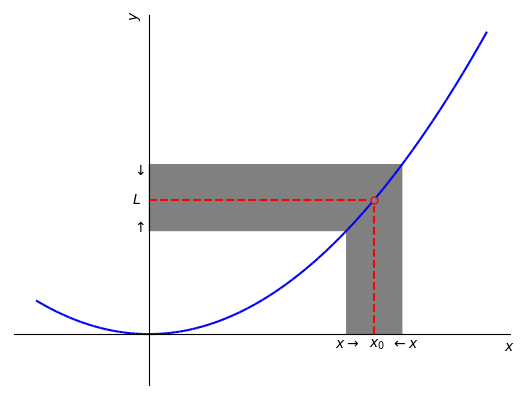
\includegraphics[width=0.7\textwidth]{./cap_lim/dados/fig_lim/fig_lim}
  \caption{Ilustração da noção de limite de uma função.}
  \label{fig:lim}
\end{figure}

\begin{ex}\label{ex:lim0}
  Consideremos a função
  \begin{equation}
    f(x) = \frac{(x^2-1)(x-2)}{(x-1)(x-2)}.
  \end{equation}
  Na Figura \ref{fig:ex_lim0}, temos um esboço do gráfico desta função.

  \begin{figure}[H]
    \centering
    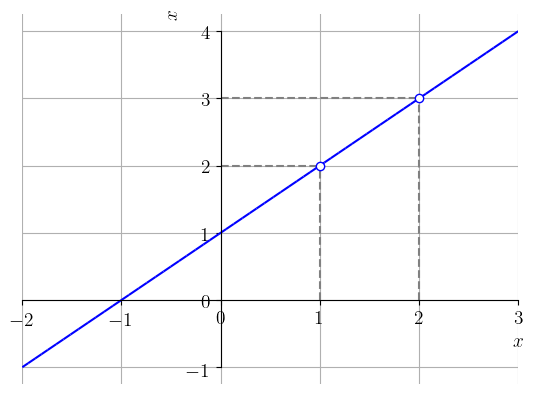
\includegraphics[width=0.7\textwidth]{./cap_lim/dados/fig_ex_lim0/fig_ex_lim0}
    \caption{Esboço do gráfico da função $f(x)$ dada no Exemplo \ref{ex:lim0}.}
    \label{fig:ex_lim0}
  \end{figure}


  Vejamos os seguintes casos:
  \begin{itemize}
  \item $\displaystyle \lim_{x\to 0} f(x) = 1 = f(0)$.
    
    \begin{tabular}{r|ccc|c|ccc}
      $x$ & $-0,01$ & $-0,001$ & $-0,0001$ & $\rightarrow 0 \leftarrow$ & $0,0001$ & $0,001$ & $0,01$\\\hline
      $f(x)$ & $0,99$ & $0,999$ & $0,9999$ & $\rightarrow 1 \leftarrow$ & $1,0001$ & $1,001$ & $1,01$
    \end{tabular}

    \ifispython
    No \sympy, podemos computar este limite com o comando
\begin{verbatim}
limit((x**2-1)*(x-2)/((x-1)*(x-2)),x,0)
\end{verbatim}
    \fi
  \item $\displaystyle \lim_{x\to 1} f(x) = 2$, embora $f(1)$ não esteja definido.
    
    \begin{tabular}{r|ccc|c|ccc}
      $x$ & $0,9$ & $0,99$ & $0,999$ & $\rightarrow 1 \leftarrow$ & $1,0001$ & $1,001$ & $1,01$\\\hline
      $f(x)$ & $1,9$ & $1,99$ & $1,999$ & $\rightarrow 2 \leftarrow$ & $2,0001$ & $2,001$ & $2,01$
    \end{tabular}
  \item $\displaystyle \lim_{x\to 2} f(x) = 3$, embora $f(2)$ também não esteja definido. Verifique!
  \end{itemize}
\end{ex}

\subsection{Limites da função constante e da função identidade}

Da noção de limite, podemos inferir que
\begin{equation}
  \lim_{x\to x_0} k = k,
\end{equation}
seja qual for a constante $k$. Veja a Figura \ref{fig:lim_funk}.

\begin{figure}[H]
  \centering
  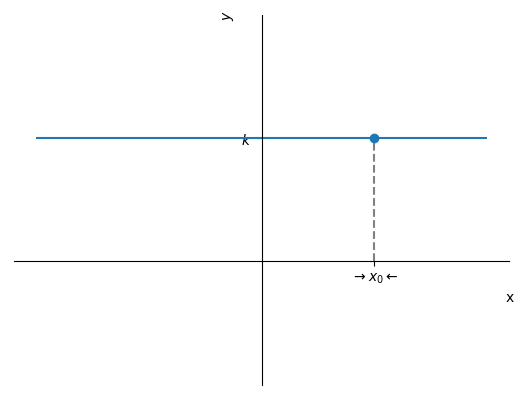
\includegraphics[width=0.7\textwidth]{./cap_lim/dados/fig_lim_funk/fig_lim_funk}
  \caption{Esboço do gráfico de uma função constante $f(x) = k$.}
  \label{fig:lim_funk}
\end{figure}

\begin{ex}
  Vejamos os seguintes casos:
  \begin{enumerate}[a)]
  \item $\displaystyle \lim_{x\to -1} 1 = 1$
  \item $\displaystyle \lim_{x\to 2} -3 = -3$
  \item $\displaystyle \lim_{x\to \pi} \sqrt{2}-e = \sqrt{2}-e$
  \end{enumerate}
\end{ex}

Também da noção de limites, podemos inferir que
\begin{equation}
  \lim_{x\to x_0} x = x_0,
\end{equation}
seja qual for o ponto $x_0$. Vejamos a Figura \ref{fig:lim_funid}.

\begin{figure}[H]
  \centering
  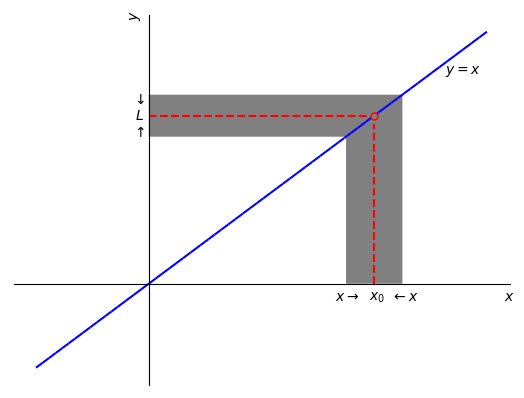
\includegraphics[width=0.7\textwidth]{./cap_lim/dados/fig_lim_funid/fig_lim_funid}
  \caption{Noção de limite para a função identidade $f(x)=x$.}
  \label{fig:lim_funid}
\end{figure}

\begin{ex}
  Vejamos os seguintes casos:
  \begin{enumerate}[a)]
  \item $\displaystyle \lim_{x\to -1} x = -1$
  \item $\displaystyle \lim_{x\to 2} x = 2$
  \item $\displaystyle \lim_{x\to \pi} x = \pi$
  \end{enumerate}
\end{ex}

\subsection*{Exercícios resolvidos}

\begin{exeresol}
  Estime o valor do limite
  \begin{equation}
    \lim_{x\to 1} e^x.
  \end{equation}
\end{exeresol}
\begin{resol}
  Da noção de limite, podemos buscar inferir o limite de uma função em um ponto $x_0$, computando seus valores próximos deste ponto. Por exemplo, construímos a seguinte tabela:
  
  \begin{tabular}{r|ccc|c|ccc}
    $x$ & $0,9$ & $0,99$ & $0,999$ & $\rightarrow 1 \leftarrow$ & $1,0001$ & $1,001$ & $1,01$\\\hline
    $f(x)$ & $2,460$ & $2,691$ & $2,716$ & $\rightarrow 2,72 \leftarrow$ & $2,719$ & $2,721$ & $2,746$
  \end{tabular}
  
  Com isso, inferimos que
  \begin{equation}
    \lim_{x\to 1} e^x \approx 2,72.
  \end{equation}
  Mais adiante, veremos que $\lim_{x\to 1} e^x = e \approx 2,718281828459045 ...$
\end{resol}

\begin{exeresol}
  Considere que uma dada função $f$ tenha o seguinte esboço de gráfico:

  \begin{center}
    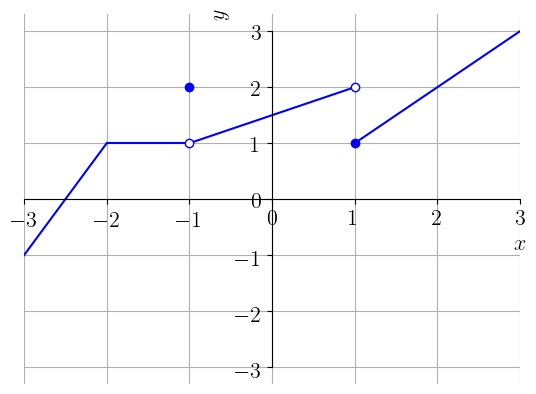
\includegraphics[width=0.7\textwidth]{./cap_lim/dados/fig_exeresol_nocaolim/fig_exeresol_nocaolim}
  \end{center}

  Então, infira o valores de
  \begin{enumerate}[a)]
  \item $\displaystyle \lim_{x\to -2} f(x)$
  \item $\displaystyle \lim_{x\to -1} f(x)$
  \item $\displaystyle \lim_{x\to 1} f(x)$
  \end{enumerate}
\end{exeresol}
\begin{resol}
  \begin{enumerate}[a)]
  \item $\displaystyle \lim_{x\to -2} f(x)$

    Para valores suficientemente próximos de $-2$ e a direita de $-2$ (i.e. $x>-2$), podemos observar que $f(x)=1$. Para tais valores de $x$ a esquerda de $-2$ (i.e. $x<-2$), vemos que os valores de $f(x)$ tornam-se próximos de $1$. Isto é, temos que os valores de $f(x)$ podemos ser tomados arbitrariamente próximos de $L=1$, se tomarmos $x$ suficientemente próximo de $-2$. Concluímos que
    \begin{equation}
      \lim_{x\to -2} = 1.
    \end{equation}

  \item $\displaystyle \lim_{x\to -1} f(x)$

    Mesmo sendo $f(-1)=2$, observamos que os valores de $f(x)$ podem ser tomados arbitrariamente próximos de $1$, se escolhemos valores de $x$ suficientemente próximos de $-1$. Logo,
    \begin{equation}
      \lim_{x\to -1} f(x) = 1.
    \end{equation}

    \item $\displaystyle \lim_{x\to 1} f(x)$

      Aqui, para valores de $x$ suficientemente próximos de $x_0=1$ e a esquerda ($x<1$), vemos que os valores de $f(x)$ são próximos de $L=2$. Entretanto, para valores de $x$ suficientemente próximos de $x_0=1$ e a direita ($x>1$), temos que os valores de $f(x)$ são próximos de $L=1$. Ou seja, não é possível escolher um valor $L$ tal que $f(x)$ esteja arbitrariamente próxima ao tomarmos $x$ suficientemente próximo de $x_0=1$, pois $L$ dependerá de $x$ estar a esquerda ou a direita de do ponto $x_0 = 1$. Concluímos que este limite não existe, e escrevemos
      \begin{equation}
        \not\exists\lim_{x\to 1} f(x).
      \end{equation}
  \end{enumerate}
\end{resol}

\subsection*{Exercícios}

\begin{exer}\label{exer:limgraf}
  Considere que uma dada função $f$ tenha o seguinte esboço de gráfico:
  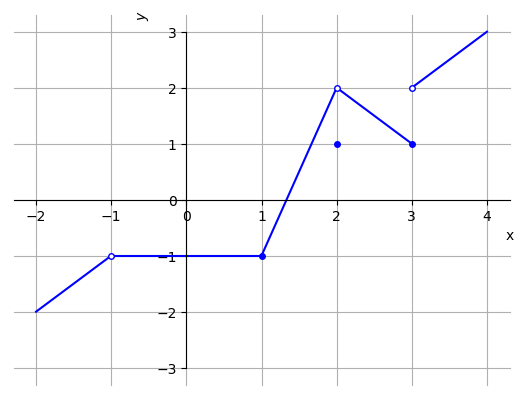
\includegraphics[width=0.8\textwidth]{./cap_lim/dados/fig_exer_limgraf/fig_exer_limgraf}

  Forneça o valor dos seguintes limites:
  \begin{enumerate}[a)]
  \item $\displaystyle \lim_{x\to -1} f(x)$
  \item $\displaystyle \lim_{x\to 1} f(x)$
  \item $\displaystyle \lim_{x\to 2} f(x)$
  \item $\displaystyle \lim_{x\to 2} f(x)$
  \item $\displaystyle \lim_{x\to 3} f(x)$
  \end{enumerate}
\end{exer}
\begin{resp}
  a)~$-1$; b)~$-1$; c)~$2$; d)~$\nexists$
\end{resp}

\begin{exer}
  Considerando a mesma função do exercício anterior (Exercícios \ref{exer:limgraf}), forneça
  \begin{enumerate}
  \item $\displaystyle \lim_{x\to -\frac{3}{2}} f(x)$
  \item $\displaystyle \lim_{x\to 0} f(x)$
  \item $\displaystyle \lim_{x\to \frac{3}{4}} f(x)$
  \end{enumerate}
\end{exer}

\begin{exer}
  Forneça o valor dos seguintes limites:
  \begin{enumerate}[a)]
  \item $\displaystyle \lim_{x\to 2} 2$
  \item $\displaystyle \lim_{x\to -2} 2$
  \item $\displaystyle \lim_{x\to 2} -3$
  \item $\displaystyle \lim_{x\to e} \pi$
  \end{enumerate}
\end{exer}
\begin{resp}
  a)~2; b)~2; c)~-3; d)~$\pi$
\end{resp}

\begin{exer}
  Forneça o valor dos seguintes limites:
  \begin{enumerate}[a)]
  \item $\displaystyle \lim_{x\to 2} x$
  \item $\displaystyle \lim_{x\to -2} x$
  \item $\displaystyle \lim_{x\to -3} x$
  \item $\displaystyle \lim_{x\to e} x$
  \end{enumerate}
\end{exer}
\begin{resp}
  a)~2; b)~-2; c)~-3; d)~$e$
\end{resp}

\section{Regras para o cálculo de limites}\label{cap_lim_sec_regras}

Sejam dados os seguintes limites
\begin{equation}
  \lim_{x\to x_0} f(x) = L_1\qquad\text{e}\qquad \lim_{x\to x_0} g(x) = L_2,
\end{equation}
com $x_0, L_1, L_2$ números reais. Então, valem as seguintes regras:
\begin{itemize}
\item Regra da multiplicação por um escalar:
  \begin{equation}
    \lim_{x\to x_0} kf(x) = k\lim_{x\to x_0} f(x) = kL_1,
  \end{equation}
  para qualquer número real $k$.
\item Regra da soma/subtração:
  \begin{equation}
    \lim_{x\to x_0} f(x) \pm g(x) = \lim_{x\to x_0} f(x) \pm \lim_{x\to x_0} g(x) = L_1 + L_2
  \end{equation}
\item Regra do produto:
  \begin{equation}
    \lim_{x\to x_0} f(x) \cdot g(x) = \lim_{x\to x_0} f(x) \cdot \lim_{x\to x_0} g(x) = L_1 \cdot L_2
  \end{equation}
\item Regra do quociente:
  \begin{equation}
    \lim_{x\to x_0} \frac{f(x)}{g(x)} = \frac{\lim_{x\to x_0} f(x)}{\lim_{x\to x_0} g(x)} = \frac{L_1}{L_2},
  \end{equation}
  desde que $L_2\neq 0$.
\item Regra da potenciação:
  \begin{equation}
    \lim_{x\to x_0} (f(x))^s = L_1^s,
  \end{equation}
  se $L_1^s$ é um número real.
\end{itemize}

Podemos usar essas regras para calcularmos limites.

\begin{ex}
  Vejamos os seguintes casos:
  \begin{enumerate}[a)]
  \item $\displaystyle \lim_{x\to -1} 2x$
  \begin{align}
    \lim_{x\to -1} 2x &= 2\lim_{x\to -1} x\\
    &= 2\cdot(-1) = -2
  \end{align}
  \ifispython
  No \sympy, podemos computar este limite com
\begin{verbatim}
limit(2*x,x,-1)
\end{verbatim}
  \fi
\item $\displaystyle \lim_{x\to 2} x^2 - 1$
  \begin{align}
    \lim_{x\to 2} x^2 - 1 &= \lim_{x\to 2} x^2 - \lim_{x\to 2} 1\\
                          &= \left(\lim_{x\to 2} x\right)^2 - \lim_{x\to 2} 1\\
    &= 2^2 - 1 = 3.
  \end{align}
  \ifispython
  No \sympy, podemos computar este limite com
\begin{verbatim}
limit(x**2-1,x,-1)
\end{verbatim}
  \fi
\item $\displaystyle \lim_{x\to 0} \sqrt{1-x^2}$.
  \begin{align}
    \lim_{x\to 0} \sqrt{1-x^2} &= \sqrt{\lim_{x\to 0} 1-x^2}\\
                                &= \sqrt{\lim_{x\to 0} 1 - \left(\lim_{x\to 0} x\right)^2}\\
                                &= \sqrt{1 - (0)^2} \\
                                &= 1.
  \end{align}
  \ifispython
  No \sympy, podemos computar este limite com
\begin{verbatim}
limit(sqrt(1-x**2),x,0)
\end{verbatim}
  \fi  
\item $\displaystyle \lim_{x\to 0} \frac{(x^2-1)(x-2)}{(x-1)(x-2)}$
  \begin{align}
    \lim_{x\to 0} \frac{(x^2-1)(x-2)}{(x-1)(x-2)} &= \frac{\lim_{x\to 0}(x^2-1)(x-2)}{\lim_{x\to 0} (x-1)(x-2)}\\
                                                  &= \frac{\lim_{x\to x_0} (x^2-1)\lim_{x\to 0}(x-2)}{\lim_{x\to 0}(x-1)\lim_{x\to 0}(x-2)}\\
    &= \frac{-2}{-2} = 1.
  \end{align}
  \end{enumerate}
\end{ex}

\begin{prop}\normalfont{(Limites de polinômios)}\label{prop:lim_poli}
  Se $p(x) = a_nx^n + a_{n-1}x^{n-1} + \cdots + a_0$, então
  \begin{equation}
    \lim_{x\to b} p(x) = p(b) = a_nb^n + a_{n-1}b^{n-1} + \cdots + a_0,
  \end{equation}
  para qualquer número real $b$ dado.
\end{prop}
\begin{dem}
  Segue das regras da soma, da multiplicação por escalar e da potenciação. Vejamos
  \begin{align}
    \lim_{x\to b} p(x) &= \lim_{x\to b} a_nx^n + a_{n-1}x^{n-1} + \cdots + a_0\\
                       &= \lim_{x\to b} a_nx^n + \lim_{x\to b} a_{n-1}x^{n-1} + \cdots + \lim_{x\to b} a_0\\
                       &= a_n\left(\lim_{x\to b} x\right)^n + a_{n-1}\left(\lim_{x\to b} x\right)^{n-1} + \cdots + a_0\\
                       &= a_nb^n + a_{n-1}b^{n-1} + \cdots + a_0 = p(b).
  \end{align}
\end{dem}

\begin{ex}
  \begin{equation}
    \lim_{x\to \sqrt{2}} 2x^4 - 2x^2 + x = 2(\sqrt{2})^4 - 2(\sqrt{2})^2 + \sqrt{2} = 4+\sqrt{2}.
  \end{equation}
  \ifispython
  No \sympy, podemos computar este limite com o comando
\begin{verbatim}
limit(2*x**4-2*x**2+x,x,sqrt(2))
\end{verbatim}
  \fi
\end{ex}

\begin{prop}\normalfont{(Limite de funções racionais)}
  Sejam $r(x) = p(x)/q(x)$ é uma função racional e $b$ um número real tal que $q(b)\neq 0$. Então,
  \begin{equation}
    \lim_{x\to b} \frac{p(x)}{q(x)} = \lim_{x\to b} \frac{p(b)}{q(b)}.
  \end{equation}
\end{prop}
\begin{dem}
  Segue da regra do limite do quociente e da Proposição \ref{prop:lim_poli}:
  \begin{align}
    \lim_{x\to b} \frac{p(x)}{q(x)} &= \frac{\lim_{x\to b} p(x)}{\lim_{x\to b} q(x)} \\
    &= \frac{p(b)}{q(b)}.
  \end{align}
\end{dem}

\begin{ex}
  \begin{equation}
    \lim_{x\to 0} \frac{(x^2-1)(x-2)}{(x-1)(x-2)} = \frac{(0^2-1)(0-2)}{(0-1)(0-2)} = 1.
  \end{equation}
  \ifispython
  No \sympy, podemos computar este limite com o comando
\begin{verbatim}
limit((x**2-1)*(x-2)/((x-1)*(x-2)),x,0)
\end{verbatim}
  \fi
\end{ex}

\subsection{Indeterminação $0/0$}

Quando $\displaystyle \lim_{x\to a} f(a)=0$ e $\displaystyle \lim_{x\to a} g(a)=0$, dizemos que
\begin{equation}
  \lim_{x\to a} \frac{f(x)}{g(x)}
\end{equation}
é uma {\bf indeterminação do tipo $0/0$}. Em vários destes casos, podemos calcular o limite eliminando o fator em comum $(x-a)$.

\begin{ex}
  \begin{align}
    \lim_{x\to 2}\frac{(x^2-1)(x-2)}{(x-1)(x-2)} = \lim_{x\to 2} \frac{x^2-1}{x-1} = 3.
  \end{align}
  \ifispython
  No \sympy, podemos computar o limite acima com
\begin{verbatim}
limit((x**2-1)*(x-2)/((x-1)*(x-2)),x,2)
\end{verbatim}
  \fi
\end{ex}

Quando o fator em comum não aparece explicitamente, podemos tentar trabalhar algebricamente de forma a explicitá-lo.

\begin{ex}
  No caso do limite
  \begin{align}
    \lim_{x\to 1} \frac{x^3-3x^2-x+3}{x^2+x-2}
  \end{align}
  temos que o denominador $p(x) = x^3-3x^2-x+3$ se anula em $x=1$, assim como o denominador $q(x) = x^2+x-2$. Assim sendo, $(x-1)$ é um fator comum entre $p(x)$ e $q(x)$. Para explicitá-lo, 
  \begin{equation}
    \frac{p(x)}{x-1} = x^2-2x-3\qquad\text{e}\qquad\frac{q(x)}{x-1} = x+2.
  \end{equation}
  \ifispython
  No \sympy, podemos computar estas divisões com os seguintes comandos
\begin{verbatim}
simplify((x**3-3*x**2-x+3)/(x-1))
simplify((x**2+x-2)/(x-1))
\end{verbatim}
  \fi
  Realizadas as divisões, temos
  \begin{equation}
    p(x) = (x-1)(x^2-2x-3)\qquad\text{e}\qquad q(x)=(x-1)(x+2).
  \end{equation}
  Com isso, temos
  \begin{align}
    \lim_{x\to 1} \frac{x^3-3x^2-x+3}{x^2+x-2} &= \lim_{x\to 1} \frac{(x-1)(x^2-2x-3)}{(x-1)(x+2)} \\
    &- \lim_{x\to 1} \frac{x^2-2x-3}{x+2} = -\frac{4}{3}.
  \end{align}
\end{ex}

\begin{ex}
  No caso de
  \begin{equation}
    \lim_{x\to 0} \frac{\sqrt{1-x}-1}{x}
  \end{equation}
  temos uma indeterminação do tipo $0/0$ envolvendo uma raiz. Neste caso, podemos calcular o limite usando de racionalização
  \begin{align}
    \lim_{x\to 0} \frac{\sqrt{1-x}-1}{x} &= \lim_{x\to 0} \frac{\sqrt{1-x}-1}{x}\frac{\sqrt{1-x}+1}{\sqrt{1-x}+1}\\
                                         &= \lim_{x\to 0} \frac{1-x-1}{x(\sqrt{1-x}+1)} \\
                                         &- \lim_{x\to 0} \frac{-x}{x(\sqrt{1-x}+1)}\\
    &= \lim_{x\to 0} \frac{-1}{\sqrt{1-x}+1} = -\frac{1}{2}.
  \end{align}
  \ifispython
  Com o \sympy, podemos computar este limite com
\begin{verbatim}
limit((sqrt(1-x)-1)/x,x,0)
\end{verbatim}
  \fi
\end{ex}

\subsection*{Exercícios resolvidos}

\begin{exeresol}
  Calcule
  \begin{equation}
    \lim_{x\to -1} \frac{x - x^2}{\sqrt{x^2+3}}.
  \end{equation}
\end{exeresol}
\begin{resol}
  Usando das propriedades de limites, calculamos
  \begin{align}
    \lim_{x\to -1} \frac{x-x^2}{\sqrt{x^2+3}} &= \frac{\lim_{x\to -1} x-x^2}{\lim_{x\to -1} \sqrt{x^2+3}} \\
                                              &= \frac{-1-(-1)^2}{\sqrt{\lim_{x\to -1} x^2+3}} \\
                                              &= \frac{-2}{\sqrt{4}} \\
                                              &= -1.
  \end{align}
\end{resol}

\begin{exeresol}
  Assumindo que o $\lim_{x\to 2} f(x) = L$ e que
  \begin{equation}
    \lim_{x\to 2} \frac{f(x)-2}{x+2} = 1,
  \end{equation}
  forneça o valor de $L$.
\end{exeresol}
\begin{resol}
  Das propriedades de limites, temos
  \begin{align*}
    \lim_{x\to 2} \frac{f(x)-2}{x+2} = 1 &\Rightarrow \frac{\lim_{x\to 2} f(x)-2}{\lim_{x\to 2} x+2} = 1\\
                                         &\Rightarrow \frac{\lim_{x\to 2} f(x) - \lim_{x\to 2} 2}{2+2} = 1\\
                                         &\Rightarrow \frac{L-2}{4} = 1\\
                                         &\Rightarrow L-2 = 4\\
                                         &\Rightarrow L = 6.
  \end{align*}
\end{resol}


\begin{exeresol}
  Calcule
  \begin{equation}
    \lim_{x\to -1} \frac{x+1}{2-\sqrt{x^2+3}}.
  \end{equation}
\end{exeresol}
\begin{resol}
  Neste caso, não podemos usar a regra do quociente, pois
  \begin{equation}
    \lim_{x\to -1} 2-\sqrt{x^2+3} = 0.
  \end{equation}
  Agora, como também temos
  \begin{equation}
    \lim_{x\to -1} x+1 = 0,
  \end{equation}
  concluímos se tratar de uma indeterminação $0/0$. Por racionalização, obtemos
  \begin{align}
    \lim_{x\to -1} \frac{x+1}{2-\sqrt{x^2+3}} &= \lim_{x\to -1} \frac{x+1}{2-\sqrt{x^2+3}}\frac{2+\sqrt{x^2+3}}{2+\sqrt{x^2+3}} \\
                                              &= \lim_{x\to -1} \frac{(x+1)(2+\sqrt{x^2+3})}{4 - (x^2+3)}\\
                                              &= \lim_{x\to -1} \frac{(x+1)(2+\sqrt{x^2+3})}{1-x^2}\\
                                              &= \lim_{x\to -1} \frac{(x+1)(2+\sqrt{x^2+3})}{(1+x)(1-x)}\\
                                              &= \lim_{x\to -1} \frac{2+\sqrt{x^2+3}}{1-x} \\
                                              &= \frac{4}{2} = 2.
  \end{align}
\end{resol}

\subsection*{Exercícios}

\begin{exer}
  Sabendo que
  \begin{equation}
    \lim_{x\to -2} f(x) = 2,
  \end{equation}
  calcule:
  \begin{enumerate}[a)]
  \item $\displaystyle \lim_{x\to 2} 2\cdot f(x)$.
  \item $\displaystyle \lim_{x\to 2} \pi\cdot f(x)$.
  \item $\displaystyle \lim_{x\to 2} -e^{\sqrt{2}}\cdot f(x)$.
  \end{enumerate}
\end{exer}
\begin{resp}
  a)~$2$; b)~$2\pi$; c)~$-2e^{\sqrt{2}}$
\end{resp}

\begin{exer}
  Considerando que
  \begin{equation}
    \lim_{x\to 3} f(x) = -2\quad\text{e}\quad\lim_{x\to 3} g(x) = \frac{1}{2},
  \end{equation}
  calcule:
  \begin{enumerate}[a)]
  \item $\displaystyle\lim_{x\to 3} f(x)+g(x)$
  \item $\displaystyle\lim_{x\to 3} g(x)-f(x)$
  \item $\displaystyle\lim_{x\to 3} f(x)-2g(x)$
  \end{enumerate}
\end{exer}
\begin{resp}
  a)~$-3/2$; b)~$-5/2$; c)~$-3$
\end{resp}

\begin{exer}
  Considerando que
  \begin{equation}
    \lim_{x\to 0} f(x) = 3\quad\text{e}\quad\lim_{x\to 0} g(x) = -2,
  \end{equation}
  calcule:
  \begin{enumerate}[a)]
  \item $\displaystyle\lim_{x\to 0} f(x)\cdot g(x)$
  \item $\displaystyle\lim_{x\to 0} g(x)\cdot (\frac{1}{2}\cdot f(x))$
  \end{enumerate}
\end{exer}
\begin{resp}
  a)~$-6$; b)~$-3$;
\end{resp}

\begin{exer}
  Considerando que
  \begin{equation}
    \lim_{x\to 0} f(x) = -2\quad\text{e}\quad\lim_{x\to 0} g(x) = -3,
  \end{equation}
  calcule:
  \begin{enumerate}[a)]
  \item $\displaystyle\lim_{x\to 0} \frac{f(x)}{g(x)}$
  \item $\displaystyle\lim_{x\to 0} \frac{g(x)}{2f(x)}$
  \end{enumerate}
\end{exer}
\begin{resp}
  a)~$2/3$; b)~$1/3$;
\end{resp}

\begin{exer}
  Considerando que
  \begin{equation}
    \lim_{x\to -1} f(x) = -1\quad\text{e}\quad\lim_{x\to -1} g(x) = 4,
  \end{equation}
  calcule:
  \begin{enumerate}[a)]
  \item $\displaystyle\lim_{x\to -1} \sqrt{g(x)}$
  \item $\displaystyle\lim_{x\to -1} \sqrt[3]{f(x)}$
  \item $\displaystyle\lim_{x\to -1} (f(x))^{\frac{4}{3}}$
  \end{enumerate}
\end{exer}
\begin{resp}
  a)~$2$; b)~$-1$; c)~$1$
\end{resp}

\begin{exer}
  Calcule os limites:
  \begin{enumerate}[a)]
  \item $\displaystyle\lim_{x\to -2} -3x$\\
  \item $\displaystyle\lim_{x\to -2} x^2-3x$\\    
  \item $\displaystyle\lim_{x\to -2} x^2-3x+\sqrt{x^2}$\\    
  \end{enumerate}
\end{exer}
\begin{resp}
  a)~$6$; b)~$10$; c)~$12$
\end{resp}

\begin{exer}
  Calcule os limites:
  \begin{enumerate}[a)]
  \item $\displaystyle\lim_{x\to -1} \frac{x}{x-1}$\\
  \item $\displaystyle\lim_{x\to -1} \frac{x^2+x-2}{x^2-3x+2}$\\    
  \end{enumerate}
\end{exer}
\begin{resp}
  a)~$1/2$; b)~$-1/3$;
\end{resp}

\begin{exer}
  Calcule os limites:
  \begin{enumerate}[a)]
  \item $\displaystyle\lim_{x\to 1} \frac{x}{x-1}$\\
  \item $\displaystyle\lim_{x\to 1} \frac{x^2+x-2}{x^2-3x+2}$\\    
  \end{enumerate}
\end{exer}
\begin{resp}
  a)~$\nexists$; b)~$\-3$;
\end{resp}

\begin{exer}
  Calcule o limite
  \begin{equation}
    \lim_{x\to 6} \frac{2-\sqrt{x-2}}{x-6}.
  \end{equation}
\end{exer}
\begin{resp}
  $-1/4$
\end{resp}


\section{Limites laterais}\label{cap_lim_sec_lateral}

Seja dada uma função $f$ definida para todo $x$ em um intervalo aberto $(a, x_0)$. O {\bf limite lateral à esquerda} de $f$ no ponto $x_0$ é denotado por
\begin{equation}
  \lim_{x\to x_0^-} f(x)
\end{equation}
e é computado tendo em vista a tendência da função apenas para pontos $x<x_0$. Em outras palavras, o
\begin{equation}
  \lim_{x\to x_0^-} f(x) = L
\end{equation}
quando $f(x)$ pode ser tomado arbitrariamente próximo de $L$, desde que tomemos $x<x_0$ suficientemente próximo de $a$. Veja a Figura \ref{fig:lim_esq}.

\begin{figure}[H]
  \centering
  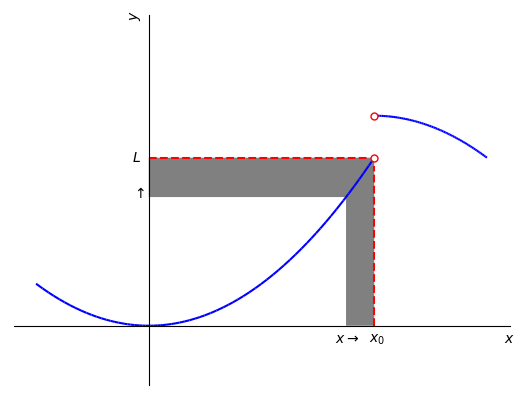
\includegraphics[width=0.7\textwidth]{./cap_lim/dados/fig_lim_esq/fig_lim_esq}
  \caption{Ilustração da noção de limite lateral à esquerda.}
  \label{fig:lim_esq}
\end{figure}

Para uma função $f$ definida para todo $x$ em um intervalo aberto $(x_0, b)$, o {\bf limite lateral à direita} de $f$ no ponto $x_0$ é denotado por
\begin{equation}
  \lim_{x\to x_0^+} f(x)
\end{equation}
e é computado tendo em vista a tendência da função apenas para pontos $x>x_0$. Em outras palavras, temos
\begin{equation}
  \lim_{x\to x_0^+} f(x) = L,
\end{equation}
quando $f(x)$ pode ser tomado arbitrariamente próximo de $L$, desde que tomemos $x>x_0$ suficientemente próximo de $x_0$. Veja a Figura \ref{fig:lim_dir}.

\begin{figure}[H]
  \centering
  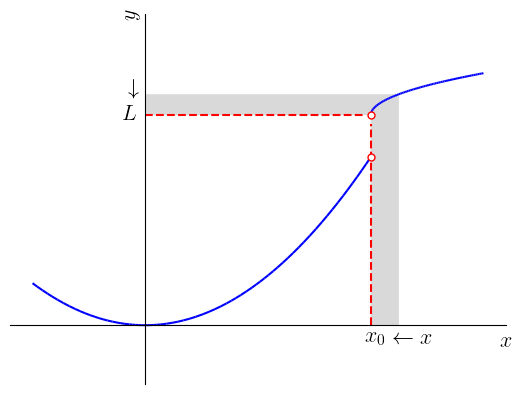
\includegraphics[width=0.7\textwidth]{./cap_lim/dados/fig_lim_dir/fig_lim_dir}
  \caption{Ilustração da noção de limite lateral à direita.}
  \label{fig:lim_dir}
\end{figure}

\begin{obs}
  Por inferência direta, temos
  \begin{equation}
    \lim_{x\to x_0^{\pm}} k = k\quad\text{e}\quad\lim_{x\to x_0^{\pm}} x = x_0,
  \end{equation}
  onde $x_0$ e $k$ são quaisquer números reais.
\end{obs}

\begin{exer}\label{ex:lim_absx}
  Vamos calcular
  \begin{equation}
    \lim_{x\to 0^-} |x|.
  \end{equation}
  Por definição, temos
  \begin{equation}
    |x| := \left\{
      \begin{array}{ll}
        x &, x\geq 0,\\
        -x &, x< 0.
      \end{array}
    \right.
  \end{equation}
  Como estamos interessados no limite lateral à esquerda de $x=0$, trabalhamos com $x<0$ e, então
  \begin{equation}
    \lim_{x\to 0^-} |x| = \lim_{x\to 0^-} -x = -\lim_{x\to 0^-} x = 0.
  \end{equation}
  
  Analogamente, calculamos
  \begin{equation}
    \lim_{x\to 0^+} |x| = \lim_{x\to 0^+} x = 0.
  \end{equation}
  Verifique!

  \ifispython
  Usando o \sympy, podemos computar os limites acima com os seguintes comandos\footnote{Veja a Observação \ref{obs:cap_lim_python}}:
\begin{verbatim}
limit(abs(x),x,0,'-')
limit(abs(x),x,0,'+')
\end{verbatim}
  \fi
\end{exer}

\begin{teo}\label{teo:lim_existe}
  Existe o limite de uma dada função $f$ no ponto $x=x_0$ e $\lim_{x\to x_0} f(x) = L$ se, e somente se, existem e são iguais a $L$ os limites laterais à esquerda e à direita de $f$ no ponto $x=x_0$.
\end{teo}

\begin{exer}
  No exemplo anterior (Exemplo \ref{ex:lim_absx}), vimos que
  \begin{equation}
    \lim_{x\to 0^-} |x| = \lim_{x\to 0^+} |x| = 0.
  \end{equation}
  Logo, pelo teorema acima (Teorema \ref{teo:lim_existe}), podemos concluir que
  \begin{equation}
    \lim_{x\to 0} |x| = 0.
  \end{equation}
\end{exer}

\begin{exer}
  Vamos verificar a existência de
  \begin{equation}
    \lim_{x\to 0} \frac{|x|}{x}.
  \end{equation}
  Começamos pelo limite lateral à esquerda, temos
  \begin{align}
    \lim_{x\to 0^-} \frac{|x|}{x} &= \lim_{x\to 0^-} \frac{-x}{x}\\
    &= \lim_{x\to 0^-} -1 = -1.
  \end{align}
  Agora, calculando o limite lateral à direta, obtemos
  \begin{align}
    \lim_{x\to 0^+} \frac{|x|}{x} &= \lim_{x\to 0^+} \frac{x}{x}\\
    &= \lim_{x\to 0^+} 1 = 1.
  \end{align}
  Como os limites laterais à esquerda e à direita são diferentes, concluímos que não existe o limite de $|x|/x$ no ponto $x=0$.

  \ifispython
  No \sympy, por padrão o limite computado é sempre o limite lateral à direita. É por isso que o comando
\begin{verbatim}
limit(abs(x)/x,x,0)
\end{verbatim}
  fornece o valor $1$ como saída.
  \fi
\end{exer}

\begin{obs}
  As regras básicas para o cálculo de limites bilaterais são estendidas para limites laterais. I.e., se
  \begin{equation}
    \lim_{x\to x_0^{\pm}} f(x) = L_1\quad\text{e}\quad\lim_{x\to x_0^{\pm}} g(x) = L_2,
  \end{equation}
  então valem a:
  \begin{itemize}
\item regra da multiplicação por um escalar:
  \begin{equation}
    \lim_{x\to x_0^{\pm}} kf(x) = k\lim_{x\to x_0^{\pm}} f(x) = kL_1,
  \end{equation}
  para qualquer número real $k$.
\item regra da soma/subtração:
  \begin{equation}
    \lim_{x\to x_0^{\pm}} f(x) \pm g(x) = \lim_{x\to x_0^{\pm}} f(x) \pm \lim_{x\to x_0^{\pm}} g(x) = L_1 + L_2
  \end{equation}
\item regra do produto:
  \begin{equation}
    \lim_{x\to x_0^\pm} f(x) \cdot g(x) = \lim_{x\to x_0^\pm} f(x) \cdot \lim_{x\to x_0^\pm} g(x) = L_1 \cdot L_2
  \end{equation}
\item regra do quociente:
  \begin{equation}
    \lim_{x\to x_0^\pm} \frac{f(x)}{g(x)} = \frac{\lim_{x\to x_0^\pm} f(x)}{\lim_{x\to x_0^\pm} g(x)} = \frac{L_1}{L_2},
  \end{equation}
  desde que $L_2\neq 0$.
\item regra da potenciação:
  \begin{equation}
    \lim_{x\to x_0^\pm} (f(x))^s = \left(\lim_{x\to x_0^\pm} f(x) \right)^s = L_1^s,
  \end{equation}
  se $L_1^s$ é um número real.
\end{itemize}
\end{obs}

\subsection*{Exercícios resolvidos}

\begin{exeresol}
  Considere que uma dada função $f$ tenha o seguinte esboço de gráfico:

  \begin{center}
    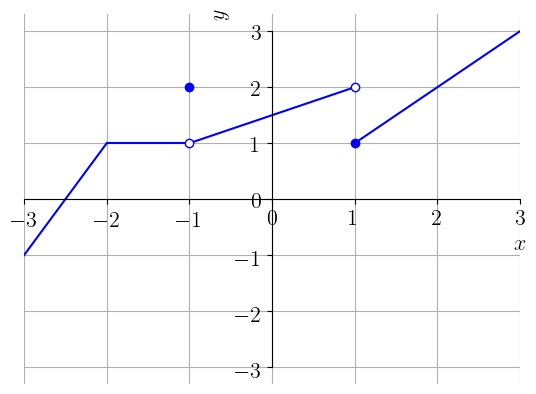
\includegraphics[width=0.7\textwidth]{./cap_lim/dados/fig_exeresol_nocaolim/fig_exeresol_nocaolim}
  \end{center}

  Então, infira o valores de
  \begin{enumerate}[a)]
  \item $\displaystyle \lim_{x\to -2^-} f(x)$
  \item $\displaystyle \lim_{x\to -1^+} f(x)$
  \item $\displaystyle \lim_{x\to 1^-} f(x)$
  \item $\displaystyle \lim_{x\to 1^+} f(x)$
  \item $\displaystyle \lim_{x\to 1} f(x)$
  \end{enumerate}
\end{exeresol}
\begin{resol}
  \begin{enumerate}[a)]
  \item $\displaystyle \lim_{x\to -2^-} f(x)$

    Para valores $x<-2$ e suficientemente próximos de $-2$, podemos observar que $f(x)$ fica arbitrariamente próximo de $1$. Concluímos que
    \begin{equation}
      \lim_{x\to -2^-} = 1.
    \end{equation}

  \item $\displaystyle \lim_{x\to -1^+} f(x)$

    Mesmo sendo $f(-1)=2$, observamos que os valores de $f(x)$ podem ser tomados arbitrariamente próximos de $1$, se escolhemos valores de $x>-1$ e suficientemente próximos de $-1$. Logo,
    \begin{equation}
      \lim_{x\to -1^+} f(x) = 1.
    \end{equation}

  \item $\displaystyle \lim_{x\to 1^-} f(x)$

    Observamos que os valores de $f(x)$ podem ser tomados arbitrariamente próximos de $2$, se escolhemos valores de $x<1$ e suficientemente próximos de $1$. Logo,
    \begin{equation}
      \lim_{x\to 1^-} f(x) = 2.
    \end{equation}
    Notamos também que, neste caso, $f(x)$ não tende para $f(1)=1$ quando $x$ tende a $1$ pela esquerda.

  \item $\displaystyle \lim_{x\to 1^+} f(x)$

    Observamos que os valores de $f(x)$ podem ser tomados arbitrariamente próximos de $1$, se escolhemos valores de $x>1$ e suficientemente próximos de $1$. Logo,
    \begin{equation}
      \lim_{x\to 1^+} f(x) = 1.
    \end{equation}
    Aqui, $f(x)\to f(1)=1$ quando $x\to 1^+$.

    \item $\displaystyle \lim_{x\to 1} f(x)$

      Nos itens anteriores, vimos que
      \begin{equation}
        2 = \lim_{x\to 1^-} f(x) \neq \lim_{x\to 1^+} f(x) = 1.
      \end{equation}
      Logo, concluímos que este limite não existe, e escrevemos
      \begin{equation}
        \not\exists\lim_{x\to 1} f(x).
      \end{equation}
  \end{enumerate}
\end{resol}

\begin{exeresol}
  Calcule $\lim_{x\to -1} f(x)$ para
  \begin{equation}
    f(x) = \left\{
      \begin{array}{ll}
        (x+1)^2-1 &, x<-1,\\
        x &, x>-1.
      \end{array}
\right.
  \end{equation}
\end{exeresol}
\begin{resol}
  A função $f$ tem comportamentos distintos para valores à esquerda e à direita de $x_0=-1$. Portanto, para calcularmos $\lim_{x\to -1} f(x)$ precisamos calcular os limites laterais. Temos:
  \begin{align}
    \lim_{x\to -1^-} f(x) &= \lim_{x\to -1^-} (x+1)^2-1\\
                          &= (-1+1)^2-1 = -1,
  \end{align}
  e
  \begin{align}
    \lim_{x\to -1^+} f(x) &= \lim_{x\to -1^+} x\\
                          &= -1.
  \end{align}
  Como ambos os limites laterais são iguais a $-1$, concluímos que
  \begin{equation}
    \lim_{x\to -1} f(x) = -1.
  \end{equation}
\end{resol}

\subsection*{Exercícios}

\begin{exer}\label{exer:limgraf}
  Considere que uma dada função $f$ tenha o seguinte esboço de gráfico:

  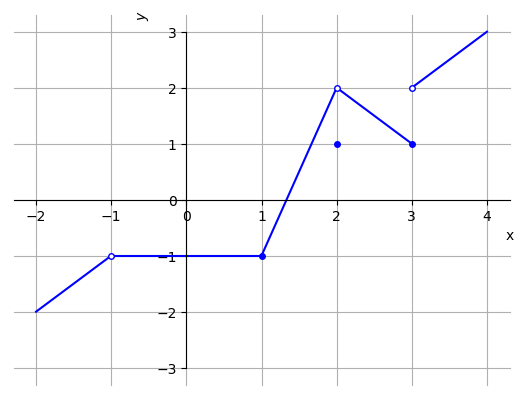
\includegraphics[width=0.8\textwidth]{./cap_lim/dados/fig_exer_limgraf/fig_exer_limgraf}

  Forneça o valor dos seguintes limites:
  \begin{enumerate}[a)]
  \item $\displaystyle \lim_{x\to 2^+} f(x)$
  \item $\displaystyle \lim_{x\to 2^-} f(x)$
  \item $\displaystyle \lim_{x\to 2} f(x)$
  \item $\displaystyle \lim_{x\to 3^+} f(x)$
  \item $\displaystyle \lim_{x\to 3^-} f(x)$
  \item $\displaystyle \lim_{x\to 3} f(x)$
  \end{enumerate}
\end{exer}
\begin{resp}
  a)~$2$; b)~$2$; c)~$2$; d)~$2$; e)~$1$; f)~$\nexists$
\end{resp}

\begin{exer}
  Sendo
  \begin{equation}
    f(x) = \left\{
      \begin{array}{ll}
        x^2+1 &, x\leq 1,\\
        2x &, x>1.
      \end{array}
    \right.
  \end{equation}
  calcule
  \begin{enumerate}[a)]
  \item $\displaystyle \lim_{x\to 1^-} f(x)$.
  \item $\displaystyle \lim_{x\to 1^+} f(x)$.
  \item $\displaystyle \lim_{x\to 1} f(x)$.
  \end{enumerate}
\end{exer}
\begin{resp}
  a)~$2$; b)~$2$; c)~$2$
\end{resp}

\begin{exer}
  Sendo
  \begin{equation}
    f(x) = \left\{
      \begin{array}{ll}
        x^2+1 &, x\leq 1,\\
        2x+1 &, x>1,
      \end{array}
    \right.
  \end{equation}
  calcule
  \begin{enumerate}[a)]
  \item $\displaystyle \lim_{x\to 1^-} f(x)$.
  \item $\displaystyle \lim_{x\to 1^+} f(x)$.
  \item $\displaystyle \lim_{x\to 1} f(x)$.
  \end{enumerate}
\end{exer}
\begin{resp}
  a)~$2$; b)~$3$; c)~$\nexists$
\end{resp}

\begin{exer}
  Calcule
  \begin{equation}
    \lim_{x\to 0^-} \frac{x}{2|x|}.
  \end{equation}
\end{exer}
\begin{resp}
  $-\frac{1}{2}$
\end{resp}

\begin{exer}
  Calcule
  \begin{equation}
    \lim_{x\to -1^+} \sqrt{1-x^2}.
  \end{equation}
  O que pode-se dizer sobre o limite à esquerda?
\end{exer}
\begin{resp}
  $0$; Não está definido, pois o domínio de $f(x)=\sqrt{1-x^2}$ é $[-1, 1]$.
\end{resp}

\section{Limites no infinito}\label{cap_lim_sec_liminf}

Limites no infinito descrevem a tendência de uma dada função $f(x)$ quando $x\to -\infty$ ou $x\to\infty$.

Dizemos que o limite de $f(x)$ é $L$ quando $x$ tende a $-\infty$, se os valores de $f(x)$ podem ser tomados arbitrariamente próximos de $L$ para valores de $x$ suficientemente pequenos. Neste caso, escrevemos
\begin{equation}
  \lim_{x\to -\infty} f(x) = L.
\end{equation}
Veja a Figura \ref{fig:lim_x-infty}.

\begin{figure}[H]
  \centering
  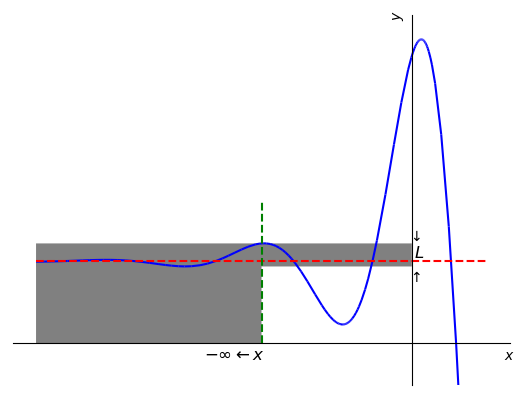
\includegraphics[width=0.7\textwidth]{./cap_lim/dados/fig_lim_x-infty/fig_lim_x-infty}
  \caption{Ilustração da noção de limite de uma função quando $x\to -\infty$.}
  \label{fig:lim_x-infty}
\end{figure}

Analogamente, dizemos que o limite de $f(x)$ é $L$ quando $x$ tende $\infty$, se os valores de $f(x)$ são arbitrariamente próximos de $L$ para valores de $x$ suficientemente grandes. Neste caso, escrevemos
\begin{equation}
  \lim_{x\to \infty} f(x) = L.
\end{equation}
Veja a Figura \ref{fig:lim_x2infty}.

\begin{figure}[H]
  \centering
  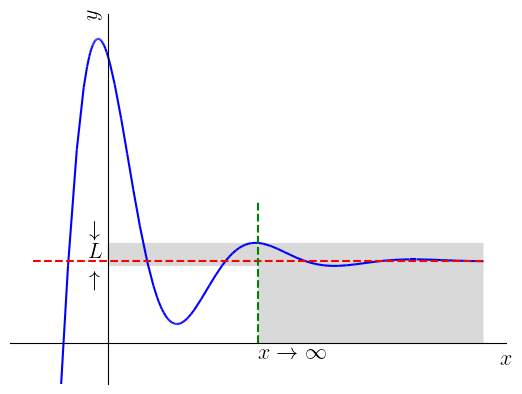
\includegraphics[width=0.7\textwidth]{./cap_lim/dados/fig_lim_x2infty/fig_lim_x2infty}
  \caption{Ilustração da noção de limite de uma função quando $x\to \infty$.}
  \label{fig:lim_x2infty}
\end{figure}


\begin{ex}
  Vamos inferir os limites de $f(x) = 1/x$ para $x\to -\infty$ e $x\to \infty$. A Figura \ref{fig:lim_xinf_1x} é um esboço do gráfico desta função.

\begin{figure}[H]
  \centering
  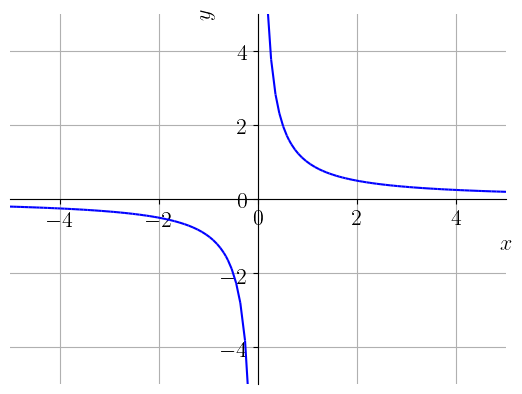
\includegraphics[width=0.7\textwidth]{./cap_lim/dados/fig_lim_xinf_1x/fig_lim_xinf_1x}
  \caption{Esboço do gráfico de $f(x) = 1/x$.}
  \label{fig:lim_xinf_1x}
\end{figure}

Observamos que quanto menores os valores de $x$, mais próximos de $0$ são os valores de $f(x)=1/x$. Daí, inferimos que
\begin{equation}
  \lim_{x\to -\infty} \frac{1}{x} = 0.
\end{equation}

Também, quanto maiores os valores de $x$, mais próximos de $0$ são os valores de $f(x)=1/x$. Com isso, podemos concluir que
\begin{equation}
  \lim_{x\to \infty} \frac{1}{x} = 0.
\end{equation}

\ifispython
Podemos computar estes limites com o \sympy, usando os seguintes comandos\footnote{Veja a Observação \ref{obs:cap_lim_python}.}:
\begin{verbatim}
limit(1/x,x,-oo)
limit(1/x,x,oo)
\end{verbatim}
\fi
\end{ex}

\begin{obs}\normalfont{(Regras para o cálculo de limites no infinito)}\label{obs:lim_regras_xinf}
Supondo que $L$, $M$ e $k$ são números reais e
\begin{equation}
  \lim_{x\to \pm\infty} f(x) = L\quad\text{e}\quad\lim_{x\to\pm\infty}g(x) = M.
\end{equation}
Então, temos as seguintes regras para limites no infinito:
\begin{itemize}
\item Regra da soma/diferença
  \begin{equation}
    \lim_{x\to\pm\infty} (f(x)\pm g(x)) = L\pm M
  \end{equation}
\item Regra do produto
  \begin{equation}
    \lim_{x\to\pm\infty} f(x)g(x) = LM
  \end{equation}
\item Regra da multiplicação por escalar
  \begin{equation}
    \lim_{x\to\pm\infty} kf(x) = kL
  \end{equation}
\item Regra do quociente
  \begin{equation}
    \lim_{x\to\pm\infty} \frac{f(x)}{g(x)} = \frac{L}{M},\quad M\neq 0.
  \end{equation}
\item Regra da potenciação
  \begin{equation}
    \lim_{x\to\pm\infty} (f(x))^k = L^k,\text{ se } L^k\in\mathbb{R}.
  \end{equation}
\end{itemize}
\end{obs}

\begin{ex}
  \begin{align}
    \lim_{x\to \infty} \frac{1}{x^2}+1 &= \lim_{x\to \infty} \frac{1}{x^2} + \lim_{x\to \infty}1 \\
                                       &= \left(\lim_{x\to\infty} \frac{1}{x}\right)^2 + 1\\
                                       &= 0^2 + 1 = 1.
\end{align}
\end{ex}

\begin{ex}\label{ex:liminf_funracio}
  Consideramos o seguinte caso
  \begin{equation}
    \lim_{x\to \infty} \frac{x^3 - 2x + 1}{2 - 3x^3}.
  \end{equation}
  Observe que não podemos usar a regra do quociente diretamente, pois, por exemplo, não existe o limite do numerador. Para contornar este problema, podemos multiplicar e dividir por $1/x^3$ (grau dominante), obtendo
  \begin{align}
    \lim_{x\to\infty} \frac{x^3 - 2x + 1}{2 - 3x^3}\cdot\frac{\frac{1}{x^3}}{\frac{1}{x^3}} = \lim_{x\to\infty} \frac{1-\frac{2}{x^2} + \frac{1}{x^3}}{\frac{2}{x^3}-3}. 
  \end{align}
  Então, aplicando a regras do quociente, da soma/subtração e da multiplicação por escalar, temos
  \begin{equation}
    \lim_{x\to\infty} \frac{x^3 - 2x + 1}{2 - 3x^3} = \lim_{x\to\infty} \frac{1-\frac{2}{x^2} + \frac{1}{x^3}}{\frac{2}{x^3}-3} = -\frac{1}{3}.
  \end{equation}
\end{ex}

\begin{obs}\label{obs:lim_xinf_racio}
  Dados dois polinômios $p(x) = a_nx^n+a_{n-1}x^{n-1}+\cdots + a_0$ e $q(x) = b_mx^m+b_{m-1}x^{m-1}+\cdots + b_0$, temos
  \begin{equation}
    \lim_{x\to \pm\infty} \frac{p(x)}{q(x)} = \frac{a_nx^n}{b_mx^m}.
  \end{equation}
\end{obs}

\begin{ex}
  Retornando ao exemplo anterior (Exemplo \ref{ex:liminf_funracio}), temos
  \begin{equation}
    \lim_{x\to\infty} \frac{x^3 - 2x + 1}{2 - 3x^3} = \lim_{x\to\infty} \frac{x^3}{-3x^3} = -\frac{1}{3}.
  \end{equation}
\end{ex}

\subsection{Assíntotas horizontais}

A reta $y = L$ é uma assíntota horizontal do gráfico da função $y = f(x)$ se
\begin{equation}
  \lim_{x\to -\infty} f(x) = L\quad\text{ou}\quad\lim_{x\to\infty} f(x) = L.
\end{equation}

\begin{ex}\label{ex:ass_hor}
  No Exemplo \ref{ex:liminf_funracio}, vimos que
  \begin{equation}
    \lim_{x\to\infty} \frac{x^3 - 2x + 1}{2 - 3x^3} = -\frac{1}{3}.
  \end{equation}
  Logo, temos que $y=-1/3$ é uma assíntota horizontal do gráfico da função
  \begin{equation}
    f(x) = \frac{x^3 - 2x + 1}{2 - 3x^3}.
  \end{equation}
  . Veja a Figura \ref{fig:ex_ass_horizon}.

      \begin{figure}[H]
      \centering
      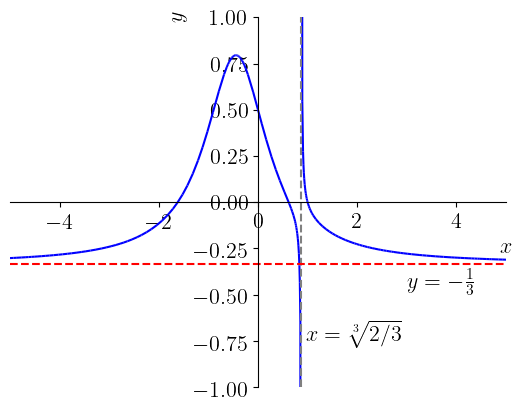
\includegraphics[width=0.7\textwidth]{./cap_lim/dados/fig_ex_ass_horizon/fig_ex_ass_horizon}
      \caption{Esboço do gráfico da função $\displaystyle f(x) = \frac{x^3 - 2x + 1}{2 - 3x^3}$.}
      \label{fig:ex_ass_horizon}
    \end{figure}

  Também, temos
  \begin{equation}
    \lim_{x\to -\infty} \frac{x^3 - 2x + 1}{2 - 3x^3} = \lim_{x\to\infty} \frac{x^3}{-3x^3} = -\frac{1}{3}.
  \end{equation}
  O que reforça que $y = -1/3$ é uma assíntota horizontal desta função.
\end{ex}

\begin{ex}\normalfont{(Função exponencial natural)}\label{ex:lim_exp_x-inf}
  \begin{equation}
    \lim_{x\to -\infty} e^x = 0,
  \end{equation}
  donde temos que $y=0$ é uma assíntota horizontal da função exponencial natural. Veja a Figura \ref{fig:lim_ex_xinf_exp}.

  \begin{figure}[H]
    \centering
    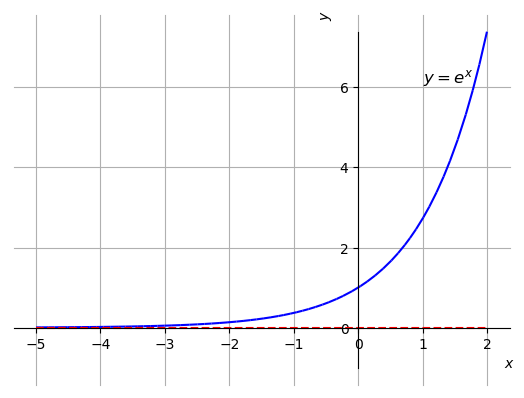
\includegraphics[width=0.7\textwidth]{./cap_lim/dados/fig_ex_xinf_exp/fig_ex_xinf_exp}
    \caption{Esboço do gráfico de $f(x)=e^x$.}
    \label{fig:lim_ex_xinf_exp}
  \end{figure}
\end{ex}

\subsection{Limite no infinito de função periódica}

Uma função $f$ é periódica quando existe um número $T$ tal que
\begin{equation}
  f(x) = f(x+T),
\end{equation}
para todo $x\in\mathbb{R}$ no domínio de $f$. As funções trigonométricas são exemplos de funções periódicas (veja a Seção \ref{cap_funcao_sec_funtri}).

O limite no infinito de funções periódicas não existe\footnote{À exceção de funções constantes.}. De fato, se $f$ não é constante, então existem números $x_1\neq x_2$ tal que $y_1=f(x_1)\neq f(x_2)=y_2$. Como a função é periódica, $f(x_1+kT)=y_1$ e $f(x_2+kT) = y_2$ para todo número inteiro $k$. Desta forma, não existe número $L$ que possamos tomar $f(x)$ arbitrariamente próxima, para todos os valores de $x$ suficientemente grandes (ou pequenos).

\begin{ex}
  Não existe
  \begin{equation}
    \lim_{x\to \infty} \sen(x),
  \end{equation}
  pois os valores de $\sen x$ oscilam periodicamente no intervalo $[-1, 1]$. Veja a Figura \ref{fig:lim_senx_xinf}.

  \begin{figure}[H]
    \centering
    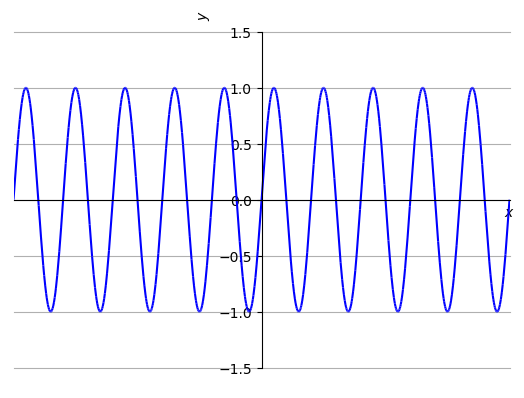
\includegraphics[width=0.7\textwidth]{./cap_lim/dados/fig_lim_senx_xinf/fig_lim_senx_xinf}
    \caption{Esboço do gráfico de $f(x)=\sen x$.}
    \label{fig:lim_senx_xinf}
  \end{figure}

  \ifispython
  No \sympy, ao computarmos $\lim_{x\to \infty} \sen x$ com o comando\footnote{Veja a Observação \ref{obs:cap_lim_python}}:
\begin{verbatim}
limit(sin(x),x,oo)
\end{verbatim}
  obtemos como saída o intervalo $[-1, 1]$, indicando que o limite não existe, pois $\sen x$ oscila indefinidamente com valores neste intervalo.
  \fi
\end{ex}


\subsection*{Exercícios resolvidos}

\begin{exeresol}
  Calcule
  \begin{equation}
    \lim_{x\to \infty} \frac{1}{x-1}+1.
  \end{equation}
\end{exeresol}
\begin{resol}
  Utilizando a regra da soma para limites no infinito, temos
  \begin{align}
    \lim_{x\to\infty} \frac{1}{x-1} + 1 &= \lim_{x\to \infty} \frac{1}{x-1} + \lim_{x\to 1} 1\\
                                        &= \lim_{x\to \infty} \left(\frac{1}{x-1}\right)+1,
  \end{align}
  observando que $\lim_{x\to \infty}1/(x-1)$ existe. De fato, o gráfico de $g(x) = 1/(x-1)$ é uma translação de uma unidade à esquerda da função $f(x)=1/x$. Uma translação horizontal finita não altera o comportamento da função para $x\to \infty$. Portanto, como $f(x)=1/x\to\infty$ quando $x\to\infty$, temos que $g(x)=f(x-1)=1/(x-1)\to\infty$ quando $x\to\infty$, i.e.
  \begin{equation}
    \lim_{x\to\infty}\frac{1}{x-1} = 0.
  \end{equation}
  Portanto, concluímos que
  \begin{equation}
    \lim_{x\to \infty} \frac{1}{x-1} + 1 = 1. 
  \end{equation}

  \ifispython
  Com o \sympy, podemos computar este limite com o seguinte comando\footnote{Veja a Observação \ref{obs:cap_lim_python}.}:
\begin{verbatim}
limit(1/(x-1)+1,x,oo)
\end{verbatim}
  \fi
\end{resol}

\begin{exeresol}
  Determine a(s) assíntota(s) horizontal(ais) do gráfico da função
  \begin{equation}
    f(x) = \frac{3 - x + 4x^4 - 10x^3}{x^2 + 2x^4 -x}.
  \end{equation}
\end{exeresol}
\begin{resol}
  Uma reta $y = L$ é assíntota horizontal do gráfico de $f$, quando
  \begin{equation}
    \lim_{x\to\pm\infty} f(x) = L.
  \end{equation}
  Começamos com $x\to-\infty$, temos
  \begin{align}
    \lim_{x\to-\infty} f(x) &= \lim_{x\to-\infty} \frac{3 - x + 4x^4 - 10x^3}{x^2 + 2x^4 -x} \\
                            &= \lim_{x\to -\infty} \frac{4x^4}{2x^4} = 2.
  \end{align}
  Logo, $y=2$ é assíntota horizontal ao gráfico de $f(x)$.

  Agora, vamos ver a tendência da função para $x\to\infty$, temos
  \begin{equation}
    \lim_{x\to\infty} f(x) = \lim_{x\to\infty} \frac{3 - x + 4x^4 - 10x^3}{x^2 + 2x^4 -x} = \frac{4}{2} = 2.
  \end{equation}
  Portanto, concluímos que $y=2$ é a única assíntota horizontal ao gráfico da função $f$.

  \ifispython
  Os seguintes comandos\footnote{Veja a Observação \ref{obs:cap_lim_python}.} do \sympy~  permitem plotar o esboço do gráfico da função $f$ (linha azul) e sua assíntota horizontal (linha vermelha):
\begin{verbatim}
f = lambda x: (3-x+4*x**4-10*x**3)/(x**2+2*x**4-x)
L = limit(f(x),x,oo)
p = plot(f(x),(x,-15,15),ylim=[-4,6],line_color="blue",show=False)
q = plot(L,(x,-15,15),line_color="red",show=False)
p.extend(q)
p.show()
\end{verbatim}
  \fi
\end{resol}

\begin{exeresol}
  Calcule
  \begin{equation}
    \lim_{x\to\infty} \frac{\sqrt{1+x^2}}{2x}.
  \end{equation}
\end{exeresol}
\begin{resol}
  Seguindo a ideia aplicada no Exemplo \ref{ex:liminf_funracio}, temos
  \begin{align}
    \lim_{x\to\infty} \frac{\sqrt{1+x^2}}{2x} &= \lim_{x\to\infty} \frac{\sqrt{1+x^2}}{x}\cdot \frac{\frac{1}{\sqrt{x^2}}}{\frac{1}{\sqrt{x^2}}} \\
                                             &= \lim_{x\to\infty} \frac{\sqrt{\frac{1}{x^2}+\frac{x^2}{x^2}}}{2\frac{x}{\sqrt{x^2}}}.
  \end{align}
  Lembramos que $\sqrt{x^2}=|x|$. Como $x\to\infty$, temos $\sqrt{x^2} = |x|=x$. Logo,
  \begin{align}
    \lim_{x\to\infty} \frac{\sqrt{\frac{1}{x^2}+\frac{x^2}{x^2}}}{2\frac{x}{\sqrt{x^2}}} &= \lim_{x\to\infty} \frac{\sqrt{\frac{1}{x^2}+\frac{x^2}{x^2}}}{2\frac{x}{|x|}}\\
                                                                                         &= \lim_{x\to\infty} \frac{\sqrt{\frac{1}{x^2}+1}}{2\frac{x}{x}}\\
                                                                                         &= \lim_{x\to\infty} \frac{1}{2}\sqrt{\frac{1}{x^2}+1}\\
                                                                                         &= \frac{1}{2}\sqrt{\lim_{x\to\infty} \frac{1}{x^2}+1}\\
                                                                                         &= \frac{1}{2}.
  \end{align}
\end{resol}

\begin{exeresol}
  Calcule
  \begin{equation}
    \lim_{x\to \infty} e^{-x}.
  \end{equation}
\end{exeresol}
\begin{resol}
  Observamos que o gráfico de $f(x)=e^{-x}$ é uma reflexão em torno do eixo $y$ do gráfico da função $g(x)=e^x$. No Exemplo \ref{ex:lim_exp_x-inf}, vimos que
  \begin{equation}
    \lim_{x\to -\infty} g(x) = \lim_{x\to -\infty} e^{x} = 0,
  \end{equation}
  logo
  \begin{equation}
    \lim_{x\to \infty} e^{-x} = \lim_{x\to \infty} g(-x) = \lim_{x\to -\infty} g(x) = 0.
  \end{equation}
  Veja o esboço do gráfico de $f(x)=e^{-x}$ na Figura \ref{fig:exeresol_lim_exp_xinf}.

  \begin{figure}[H]
    \centering
    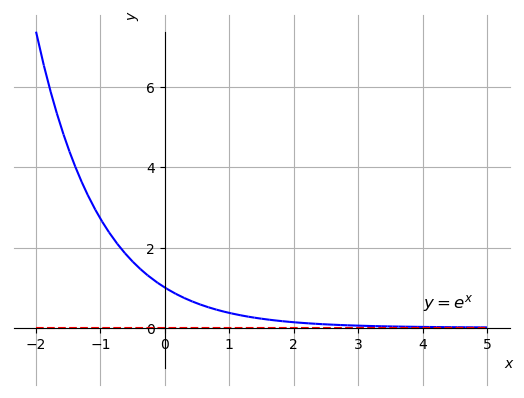
\includegraphics[width=0.7\textwidth]{./cap_lim/dados/fig_exeresol_lim_exp_xinf/fig_exeresol_lim_exp_xinf}
    \caption{Esboço do gráfico de $f(x)=e^{-x}$.}
    \label{fig:exeresol_lim_exp_xinf}
  \end{figure}  

  \ifispython
  Com o \sympy, podemos computar este limite com o seguinte comando\footnote{Veja a Observação \ref{obs:cap_lim_python}.}:
\begin{verbatim}
limit(exp(-x),x,oo)
\end{verbatim}
  \fi
\end{resol}

\subsection*{Exercícios}

\begin{exer}
  Calcule
  \begin{equation}
    \lim_{x\to -\infty} 2 - \frac{1}{x+1}.
  \end{equation}
\end{exer}
\begin{resp}
  $2$
\end{resp}

\begin{exer}
  Calcule
\end{exer}
\begin{enumerate}[a)]
\item $\displaystyle \lim_{x\to -\infty} e^x+1$
\item $\displaystyle \lim_{x\to \infty} 3 + e^{-x}$
\item $\displaystyle \lim_{x\to \infty} 2e^{-x}-1$
\item $\displaystyle \lim_{x\to -\infty} e-e^{-x}$
\end{enumerate}
\begin{resp}
  a)~$1$; b)~$3$; c)~$-1$; d)~$e$
\end{resp}

\begin{exer}
  Calcule
  \begin{equation}
    \lim_{x\to -\infty} \cos x.
  \end{equation}
\end{exer}
\begin{resp}
  não existe.
\end{resp}

\begin{exer}
  Calcule:
  \begin{enumerate}[a)]
  \item $\displaystyle\lim_{x\to \infty} \sqrt{1+e^{-x}}$.
  \item $\displaystyle\lim_{x\to -\infty} \frac{1-2x}{x+3} -e^{x} - 1$.
  \end{enumerate}
\end{exer}

\section{Limites infinitos}\label{cap_lim_sec_lim_inf}

O limite de uma função nem sempre existe. Entretanto, em muitos destes casos, podemos concluir mais sobre a tendência da função. Por exemplo, dizemos que o limite de uma dada função $f(x)$ é infinito quando $x$ tende a um número $x_0$, quando $f(x)$ torna-se arbitrariamente grande para todos os valores de $x$ suficientemente próximos de $x_0$, mas $x\neq 0$. Neste caso, escrevemos
\begin{equation}
  \lim_{x\to x_0} f(x) = \infty.
\end{equation}
A Figura \ref{fig:liminf}, é uma ilustração de $f(x)\to\infty$ quando $x\to x_0$.

\begin{figure}[H]
  \centering
  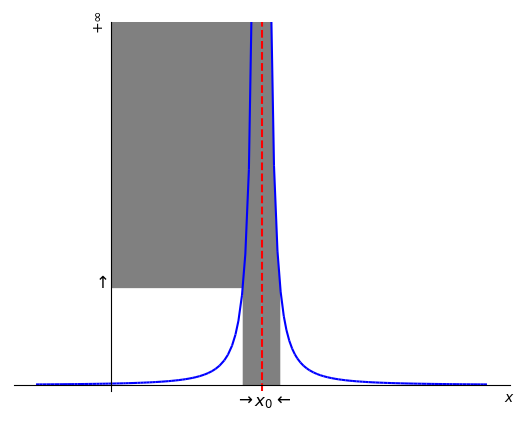
\includegraphics[width=0.7\textwidth]{./cap_lim/dados/fig_liminf/fig_liminf}
  \caption{Ilustração de $f(x)\to\infty$ quando $x\to x_0$.}
  \label{fig:liminf}
\end{figure}


\begin{ex}
  Vejamos o caso de
  \begin{equation}
    \lim_{x\to 0} \frac{1}{x^2}.
  \end{equation}
  Ao tomarmos $x$ próximo de $x_0=0$, obtemos os seguintes valores de $f(x)$:
  \begin{center}
    \begin{tabular}[H]{l|ccc|c|ccc}
      x & $-10^{-1}$ & $-10^{-2}$ & $-10^{-3}$ & $\rightarrow 0 \leftarrow$ & $10^{-3}$ & $10^{-2}$ & $10^{-1}$ \\\hline
      f(x) & $-10^{2}$ & $-10^{4}$ & $-10^{6}$ & $\rightarrow \infty \leftarrow$ & $10^{6}$ & $10^{4}$ & $10^{2}$
    \end{tabular}
  \end{center}
  Veja o esboço do gráfico de $f(x)$ na Figura \ref{fig:ex_liminf_1x2}.

\begin{figure}[H]
  \centering
  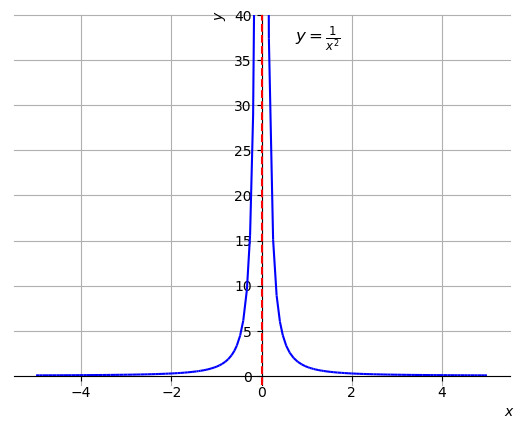
\includegraphics[width=0.7\textwidth]{./cap_lim/dados/fig_ex_liminf_1x2/fig_ex_liminf_1x2}
  \caption{Esboço do gráfico de $f(x)=1/x^2$.}
  \label{fig:ex_liminf_1x2}
\end{figure}  

  Podemos concluir que os valores de $f(x)$ podem ser tomados arbitrariamente grandes ao escolhermos qualquer $x$ suficientemente próximo de $0$, com $x\neq 0$. I.e.,
  \begin{equation}
    \lim_{x\to 0}\frac{1}{x^2} = \infty.
  \end{equation}

  \ifispython
  No \sympy, podemos computar este limite com o seguinte comando\footnote{Veja a Observação \ref{obs:cap_lim_python}.}:
\begin{verbatim}
limit(1/x**2,x,0)
\end{verbatim}
  Atenção! Na verdade, este comando computa o limite lateral à direita. Na sequência, discutimos sobre limites laterais infinitos.
  \fi
\end{ex}

Definimos os limites laterais infinitos
\begin{equation}
  \lim_{x\to x_0^-} f(x) = \infty\quad\text{e}\quad\lim_{x\to x_0^+} f(x) = \infty.
\end{equation}
No primeiro caso, os valores de $f(x)$ são arbitrariamente grandes conforme os valores de $x\to x_0$ e $x<x_0$. No segundo caso, os valores de $f(x)$ são arbitrariamente grandes conforme os valores de $x\to x_0$ e $x>x_0$.

\begin{ex}
  \begin{equation}
    \lim_{x\to 1^+} \frac{1}{x-1} = \infty.
  \end{equation}
  De fato, conforme tomamos valores de $x$ próximos de $1$, com $x>1$, os valores de $f(x) = 1/(x-1)$ tornam-se cada vez maiores. Veja o esboço do gráfico de $f(x)$ na Figura \ref{fig:ex_liminf_1x}.

\begin{figure}[H]
  \centering
  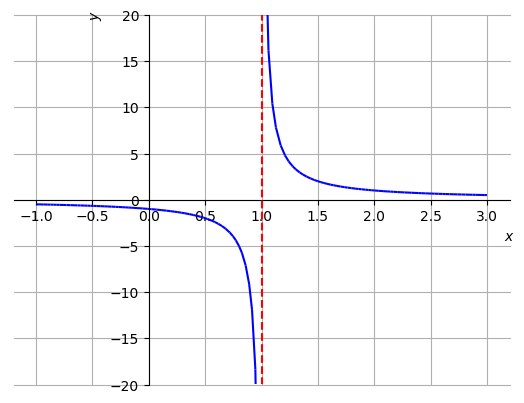
\includegraphics[width=0.7\textwidth]{./cap_lim/dados/fig_ex_liminf_1x/fig_ex_liminf_1x}
  \caption{Esboço do gráfico de $f(x)=1/(x-1)$.}
  \label{fig:ex_liminf_1x}
\end{figure}  

\ifispython
  No \sympy, podemos computar este limite com o seguinte comando\footnote{Veja a Observação \ref{obs:cap_lim_python}.}:
\begin{verbatim}
limit(1/(x-1),x,0,'+')
\end{verbatim}
\fi
\end{ex}


Analogamente a definição de limite infinito, dizemos que o limite de uma dada função $f(x)$ é menos infinito quando $x$ tende a $x_0$, quando $f(x)$ torna-se arbitrariamente pequeno para valores de $x$ suficientemente próximos de $x_0$, com $x\neq x_0$. Neste caso, escrevemos
\begin{equation}
  \lim_{x\to x_0} f(x) = -\infty.
\end{equation}
De forma similar, definimos os limites laterais $f(x)\to -\infty$ quando $x\to x_0^{\pm}$.

\begin{ex}
  Observe que
  \begin{equation}
    \nexists \lim_{x\to 0} \frac{1}{x}
  \end{equation}
  e que não podemos concluir que este limite é $\infty$ ou $-\infty$. Isto ocorre, pois
  \begin{equation}
    \lim_{x\to 0^-} \frac{1}{x} = -\infty\quad\text{e}\quad\lim_{x\to 0^+} \frac{1}{x} = +\infty.
  \end{equation}
\end{ex}

\begin{ex}
  \begin{equation}
    \lim_{x\to -1} \frac{-1}{(x+1)^2} = -\infty.
  \end{equation}
  De fato, podemos inferir este limite a partir do gráfico da função $f(x) = 1/(x+1)^2$. Este é uma translação de uma unidade à esquerda do gráfico de $y = 1/x^2$, seguida de uma reflexão em torno de eixo $x$. Veja a Figura \ref{fig:ex_liminf-1x2}.

  \begin{figure}[H]
    \centering
    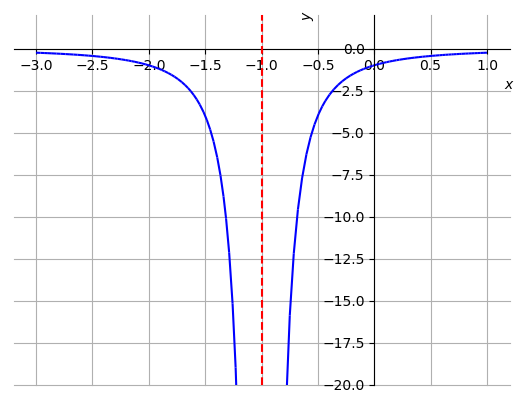
\includegraphics[width=0.7\textwidth]{./cap_lim/dados/fig_ex_liminf-1x2/fig_ex_liminf-1x2}
    \caption{Esboço do gráfico de $f(x)=-1/(x+1)^2$.}
    \label{fig:ex_liminf-1x2}
  \end{figure}

  \ifispython
  No \sympy, podemos computar este limite com o seguinte comando\footnote{Veja a Observação \ref{obs:cap_lim_python}.}:
\begin{verbatim}
limit(-1/(x+1)**2,x,-1)
\end{verbatim}
  Novamente, observamos que este comando computa apenas o limite lateral à direita.
  \fi
\end{ex}

\subsection{Assíntotas verticais}

Uma reta $x=x_0$ é uma {\bf assíntota vertical} do gráfico de uma função $y = f(x)$ se
\begin{equation}
  \lim_{x\to x_0^-} f(x) = \pm\infty\quad\text{ou}\quad\lim_{x\to x_0^+} f(x) = \pm\infty.
\end{equation}

\begin{ex}
  O gráfico da função $f(x)=-1/|x|$ tem uma assíntota vertical em $x=0$, pois
  \begin{equation}
    \lim_{x\to 0} \frac{-1}{|x|} = -\infty.
  \end{equation}
  Veja o esboço de seu gráfico na Figura \ref{fig:ex_lim_assvert_1}.

  \begin{figure}[H]
    \centering
    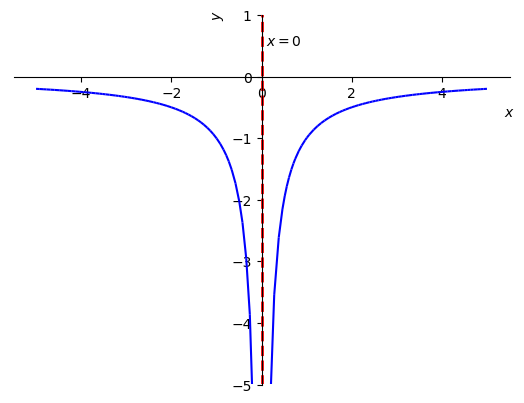
\includegraphics[width=0.7\textwidth]{./cap_lim/dados/fig_ex_lim_assvert_1/fig_ex_lim_assvert_1}
    \caption{Esboço do gráfico de $f(x)=-1/|x|$.}
    \label{fig:ex_lim_assvert_1}
  \end{figure}  
\end{ex}

\begin{ex}
  A função $\displaystyle f(x) = \frac{x^3 + 2x^2 - 4x - 8}{x^2 - 1}$ não está definida para valores de $x$ tais que seu denominador se anule, i.e.
    \begin{equation}
      x^2 - 1 = 0 \Rightarrow x_0=-1\quad\text{ou}\quad x_1=1.
    \end{equation}
    Nestes pontos o gráfico de $f$ pode ter assíntotas verticais. De fato, temos
    \begin{equation}
      \lim_{x\to -1^\pm} \frac{x^3 + 2x^2 - 4x - 8}{x^2-1} =  \pm\infty,
    \end{equation}
    e, também, temos
    \begin{equation}
      \lim_{x\to -1^\pm} \frac{x^3 + 2x^2 - 4x - 8}{x^2-1} =  \mp\infty,      
    \end{equation}
    Com isso, temos que as retas $x=-1$ e $x=1$ são assíntotas verticais ao gráfico da função $f$. Veja a Figura \ref{fig:ex_lim_assvert_racio} para o esboço do gráfico desta função.

    \begin{figure}[H]
      \centering
      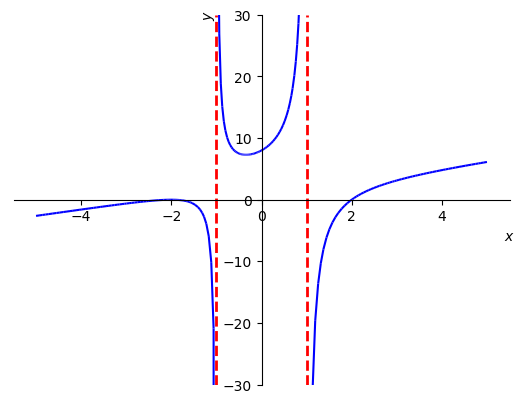
\includegraphics[width=0.7\textwidth]{./cap_lim/dados/fig_ex_lim_assvert_racio/fig_ex_lim_assvert_racio}
      \caption{Esboço do gráfico da função $\displaystyle f(x) = \frac{x^3 + 2x^2 - 4x - 8}{x^2 - 1}$.}
      \label{fig:ex_lim_assvert_racio}
    \end{figure}
\end{ex}

\begin{ex}\normalfont{(Função logarítmica)}
  A função logarítmica natural $y = \ln x$ é tal que
  \begin{equation}
    \lim_{x\to 0^+} \ln x = -\infty
  \end{equation}
  i.e., $x=0$ é uma assíntota vertical ao gráfico de $\ln x$. Isto decorre do fato de $y = \ln x$ ser a função inversa de $y = e^x$ e, esta, ter uma assíntota horizontal $y=0$\footnote{Veja o Exemplo \ref{ex:lim_exp_x-inf}.}. A Figura \ref{fig:ex_lim_assvert_lnx} é um esboço do gráfico da função  $\ln x$.

    \begin{figure}[H]
      \centering
      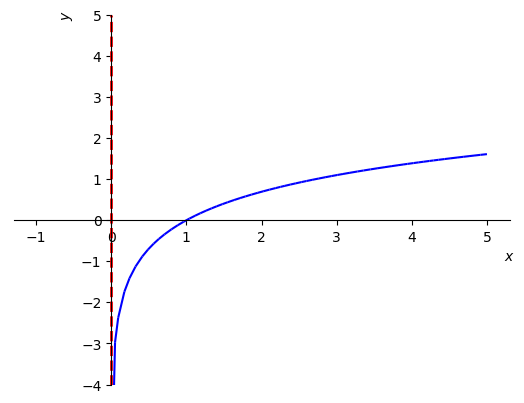
\includegraphics[width=0.7\textwidth]{./cap_lim/dados/fig_ex_lim_assvert_lnx/fig_ex_lim_assvert_lnx}
      \caption{Esboço do gráfico da função logaritmo natural.}
      \label{fig:ex_lim_assvert_lnx}
    \end{figure}  
\end{ex}

\begin{ex}
  As funções trigonométricas $y = \sec x$ e $\displaystyle y = \tg x$ têm assíntotas verticais $x = (2k+1)\frac{\pi}{2}$ para $k$ inteiro. Veja as Figuras \ref{fig:co_tg_graficos}.
\end{ex}

\begin{ex}
  As funções trigonométricas $y = \cosec x$ e $\displaystyle y = \cotg x$ têm assíntotas verticais $x = k\pi$ para $k$ inteiro. Veja as Figuras \ref{fig:co_sec_graficos}.
\end{ex}

\subsection{Assíntotas oblíquas}

Além de assíntotas horizontais e verticais, gráficos de funções podem ter assintota oblíquas. Isto ocorre, particularmente, para funções racionais cujo grau do numerador é maior que o do denominador.

\begin{figure}[H]
  \centering
  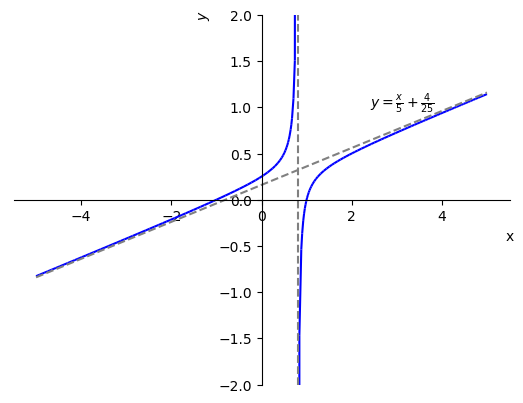
\includegraphics[width=0.7\textwidth]{./cap_lim/dados/fig_ex_ass_obl/fig_ex_ass_obl}
  \caption{Esboço do gráfico da função $\displaystyle f(x) = \frac{x^2-1}{5x-4}$.}
  \label{fig:ex_ass_obl}
\end{figure}


\begin{ex}
  Consideremos a função racional
  \begin{equation}
    f(x) = \frac{x^2-1}{5x-4}.
  \end{equation}
  Para buscarmos determinar a assíntota oblíqua desta função, dividimos o numerador pelo denominador, de forma a obtermos
  \begin{equation}
    f(x) = \underbrace{\left(\frac{x}{5}+\frac{4}{25}\right)}_{\text{quociente}} + \underbrace{\frac{-\frac{9}{25}}{5x-4}}_{\text{resto}}.
  \end{equation}
  Observamos, agora, que o resto tende a zero quando $x\to\pm\infty$, i.e. $\displaystyle f(x)\to \frac{x}{5}+\frac{4}{25}$ quando $x\to\pm\infty$. Com isso, concluímos que $\displaystyle y = \frac{x}{5}+\frac{4}{25}$ é uma assíntota oblíqua ao gráfico de $f(x)$. Veja a Figura \ref{fig:ex_ass_obl}.
\end{ex}

\begin{obs}
  Analogamente à assintotas oblíquas, podemos ter outros tipos de assíntotas determinadas por funções de diversos tipos, por exemplo, assíntotas quadráticas.
\end{obs}

\subsection{Limites infinitos no infinito}

Escrevemos
\begin{equation}
  \lim_{x\to\infty} f(x)=\infty,
\end{equation}
quando os valores da função $f$ são arbitrariamente grandes para todos os valores de $x$ suficientemente grandes. De forma análoga, definimos
\begin{equation}
  \lim_{x\to -\infty} f(x)=\infty,\quad\lim_{x\to \infty} f(x)=-\infty\quad\text{e}\quad\lim_{x\to -\infty} f(x)=-\infty.
\end{equation}

\begin{ex}
  Vejamos os seguintes casos:
  \begin{enumerate}[a)]
  \item $\displaystyle\lim_{x\to\infty} x^2 = \infty$
  \item $\displaystyle\lim_{x\to -\infty} x^2 = \infty$
  \item $\displaystyle\lim_{x\to -\infty} x^3 = -\infty$
  \item $\displaystyle\lim_{x\to \infty} e^x = \infty$
  \item $\displaystyle\lim_{x\to \infty} \ln x = \infty$
  \item $\displaystyle\lim_{x\to -\infty} e^{-x} = \infty$
  \end{enumerate}
\end{ex}

\subsection*{Exercícios resolvidos}

\begin{exeresol}
  Calcule
  \begin{equation}
    \lim_{x\to 1^-} \frac{x-2}{1-x}. 
  \end{equation}
\end{exeresol}
\begin{resol}
  Observamos que $y = 1-x\to 0^+$ quando $x\to 1^-$. Assim, fazendo a mudança de variável $y = x-1$, temos
  \begin{equation}
    \lim_{x\to 1^-} \frac{x-2}{1-x} = \lim_{y\to 0^+} \frac{y+1-2}{y} = \lim_{y\to 0^+} \frac{y-1}{y} = -\infty.
  \end{equation}

  \ifispython
  Podemos usar o seguinte comando \sympy\footnote{Veja a Observação \ref{obs:cap_lim_python}.} para computar este limite:
\begin{verbatim}
limit((x-2)/(1-x),x,1,'-')
\end{verbatim}
  \fi
\end{resol}

\begin{exeresol}
  Calcule
  \begin{equation}
    \lim_{x\to 1} \ln |x-1|.
  \end{equation}
\end{exeresol}
\begin{resol}
  Começamos observando que
  \begin{equation}
    \ln |x-1| = \left\{
      \begin{array}{ll}
        \ln(1-x) &, x < 1,\\
        \ln(x-1) &, x > 1.
      \end{array}
    \right.
  \end{equation}
  Então, calculando o limite lateral à esquerda, temos
  \begin{align*}
    \lim_{x\to 1^-} \ln |x-1| &= \lim_{x\to 1^-} \ln(1-x)\\
                              &= \lim_{y\to 0^+} \ln y = -\infty\footnote{Observe que $1-x\to 0^+$ quando $x\to 1^-$.}.
  \end{align*}
  Por outro lado, temos
  \begin{align*}
    \lim_{x\to 1^+} \ln |x-1| &= \lim_{x\to 1^+} \ln(x-1)\\
                              &= \lim_{y\to 0^+} \ln y = -\infty\footnote{Observe que $x-1\to 0^+$ quando $x\to 1^+$.}.
  \end{align*}
  Portanto, concluímos que
  \begin{equation}
    \lim_{x\to 1} \ln |x-1| = -\infty.
  \end{equation}

  \ifispython
  Podemos usar os seguintes comandos \sympy\footnote{Veja a Observação \ref{obs:cap_lim_python}.} para computar os limites laterais:
\begin{verbatim}
limit(log(abs(x-1)),x,1,'-')
limit(log(abs(x-1)),x,1,'+')
\end{verbatim}
  \fi
\end{resol}

\begin{exeresol}
  Calcule
  \begin{equation}
    \lim_{x\to \infty} \frac{x^3+2x^2-4x-8}{x^2-1}.
  \end{equation}
\end{exeresol}
\begin{resol}
  Tratando-se de uma função racional, temos\footnote{Veja a Observação \ref{obs:lim_xinf_racio}. Veja, também, o gráfico desta função na Figura \ref{fig:ex_lim_assvert_racio}.}
  \begin{equation}
    \lim_{x\to \infty} \frac{x^3+2x^2-4x-8}{x^2-1} = \lim_{x\to\infty} \frac{x^3}{x^2} = \lim_{x\to \infty} x = \infty.    
  \end{equation}
\end{resol}

\begin{exeresol}
  Calcule
  \begin{equation}
    \lim_{x\to \infty} e^{1-x^2}.
  \end{equation}
\end{exeresol}
\begin{resol}
  Observamos que $1-x^2\to -\infty$ quando $x\to \infty$. Desta forma, fazendo a mudança de variáveis $y = 1 - x^2$, temos
  \begin{equation}
    \lim_{x\to\infty} e^{1-x^2} = \lim_{y\to -\infty} e^y = 0.
  \end{equation}
\end{resol}

\subsection*{Exercícios}

\begin{exer}
  Calcule
  \begin{equation}
    \lim_{x\to -1} \frac{x^2 - 3x + 2}{x^2 + 2x + 1}.
  \end{equation}
\end{exer}
\begin{resp}
  $\infty$
\end{resp}

\begin{exer}
  Determine as assíntotas verticais ao gráfico da função
  \begin{equation}
    f(x) = \frac{8}{x^2-4}.
  \end{equation}
\end{exer}
\begin{resp}
  $x=2$; $x=-2$
\end{resp}

\begin{exer}
  Calcule
  \begin{equation}
    \lim_{x\to -\infty} e^{x^2-1}.
  \end{equation}
\end{exer}
\begin{resp}
  $\infty$
\end{resp}

\section{Continuidade}\label{cap_lim_sec_cont}

Dizemos que uma {\bf função} $f$ é {\bf contínua} em um ponto $x_0$, quando $f(x_0)$ está definida, existe o limite $\displaystyle \lim_{x\to x_0} f(x)$ e
\begin{equation}
  \lim_{x\to x_0} f(x) = f(x_0).
\end{equation}
Usando de limites laterais, definimos os conceitos de {\bf função contínua à esquerda} ou à {\bf direta}. Quando a {\bf função} $f$ não é contínua em um dado ponto $x_0$, dizemos que $f$ é {\bf descontínua} neste ponto.

\begin{ex}\label{ex:conta}
  Consideremos a seguinte função
  \begin{equation}
    f(x) = \left\{
      \begin{array}{ll}
        \frac{x-2}{(x+1)(x-2)} &, x\neq 2,\\
        -4 &, x=2.
      \end{array}
\right.
\end{equation}
Na Figura \ref{fig:ex_conta}, temos um esboço do gráfico de $f$.

\begin{figure}[H]
  \centering
  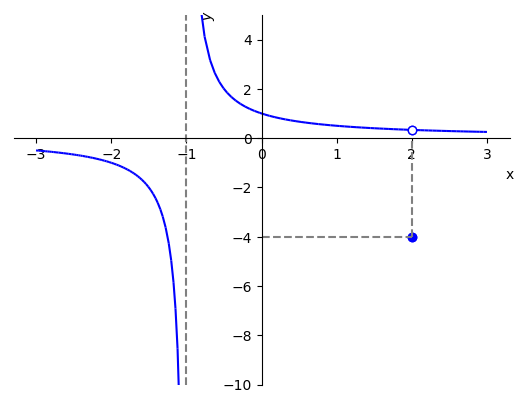
\includegraphics[width=0.7\textwidth]{./cap_lim/dados/fig_ex_conta/fig_ex_conta}
  \caption{Esboço do gráfico da função $f$ definida no Exemplo \ref{ex:conta}.}
  \label{fig:ex_conta}
\end{figure}

Vejamos a continuidade desta função nos seguintes pontos:
\begin{enumerate}[a)]
\item $x=-2$. Neste ponto, temos $f(-2) = -1$ e
  \begin{equation}
    \lim_{x\to -2} \frac{x-2}{(x+1)(x-2)} = \frac{-4}{-1\cdot(-4)} = -1 = f(-2).
  \end{equation}
  Com isso, concluímos que $f$ é contínua no ponto $x=-2$.
\item $x=-1$. Neste ponto,
  \begin{equation}
    f(-1) = \frac{(x-2)}{(x+1)(x-2)} = \frac{1}{x-1} = \frac{1}{0}
  \end{equation}
  logo, f(-1) não está definido e, portanto, $f$ é descontínua neste ponto. Observemos que $f$ tem uma assíntota vertical em $x=-1$, verifique!
\item $x=2$. Neste ponto, temos $f(2)=-4$ e
  \begin{equation}
    \lim_{x\to 2} \frac{x-2}{(x+1)(x-2)} = \lim_{x\to 2} \frac{1}{x+1} = \frac{1}{3} \neq f(2).
  \end{equation}
  Portanto, concluímos que $f$ é descontínua em $x=2$.
\end{enumerate}
\end{ex}

Uma função $f$ é dita ser {\bf contínua em um intervalo} $(a, b)$, quando $f$ é contínua em todos os pontos $x_0\in (a, b)$. Para intervalos, $[a, b)$, $(a, b]$ ou $[a, b]$, empregamos a noção de continuidade lateral nos pontos de extremos fechados dos intervalos. Quando uma função é contínua em $(-\infty, \infty)$, dizemos que ela é {\bf contínua em toda parte}.

\begin{ex}\normalfont{(Continuidade da função valor absoluto.)}
  A função valor absoluto é contínua em toda parte. De fato, ela é definida por
  \begin{equation}
    |x| = \left\{
      \begin{array}{ll}
        x &, x\geq 0,\\
        -x &, x<0.
      \end{array}
    \right.
  \end{equation}
  Veja o esboço do gráfico desta função na Figura \ref{fig:cap_funcao_funabs}.
  
  Observamos que para $x\in(-\infty, 0)$ temos $|x| = x$ que é contínua para todos estes valores de $x$. Também, para $x\in(0,\infty)$ temos $|x|=-x$ que é contínua para todos estes valores de $x$. Agora, em $x=0$, temos $|0|=0$ e
  \begin{align}
    \lim_{x\to 0^+} |x| &= \lim_{x\to 0^+} x = 0,\\
    \lim_{x\to 0^-} |x| &= \lim_{x\to 0^-} -x = 0.
  \end{align}
  Logo,
  \begin{equation}
    \lim_{x\to 0} |x| = 0 = |0|.
  \end{equation}
  Com tudo isso, concluímos que a função valor absoluto é contínua em toda parte.
\end{ex}

\begin{prop}\normalfont{(Propriedades de funções contínuas)}
  Se $f$ e $g$ são funções contínuas em $x=c_0$ e $k$ um número real, então também são contínuas em $x=x_0$ as funções:
  \begin{itemize}
  \item $kf$
  \item $f\pm g$
  \item $f\cdot g$
  \item $f/g$, se $g(x_0)\neq 0$
  \item $f^k$, se existe $f^k(x_0)$.
  \end{itemize}
\end{prop}

\begin{ex}
  {\bf Polinômios são contínuos em toda parte}. Isto é, se $p(x) = a_nx^n+a_{n-1}x^{n-1}+\cdots+a_1x+a_0$, então
  \begin{equation}
    \lim_{x\to x_0} p(x) = p(x_0),
  \end{equation}
  para qualquer $x_0\in\mathbb{R}$. Por exemplo,
  \begin{equation}
    \lim_{x\to -1} 2 - x^2 + x^5 = 2 - (-1)^2 + (-1)^5 = 0.
  \end{equation}
\end{ex}

\begin{ex}
  {\bf Funções racionais $r(x) = p(x)/q(x)$ são contínuas em todos os pontos de seus domínios}. Por exemplo, a função racional
  \begin{equation}
    f(x) = \frac{x-1}{x^2-1},
  \end{equation}
  é descontínua nos pontos
  \begin{equation}
    x^2-1 = 0 \Rightarrow x = \pm 1,
  \end{equation}
  pois $f$ não está definida nestes pontos. Agora, para $x_0\neq 1$ e $x_0\neq -1$, temos
  \begin{align}
    \lim_{x\to x_0} f(x) &= \lim_{x\to x_0} \frac{x-1}{x^2-1}\\
                         &= \frac{x_0-1}{x_0^2-1} = f(x_0).
  \end{align}
  Por exemplo,
  \begin{equation}
    \lim_{x\to 0} f(x) = \frac{0-1}{0^2-1} = 1 = f(0).
  \end{equation}
  Ou seja, $f$ é contínua nos intervalos $(-\infty, -1) \cup (-1, 1) \cup (1, \infty)$, que coincide com seu domínio.
\end{ex}

\begin{obs}
  São contínuas em todo seu domínio as funções potência, polinomiais, racionais, trigonométricas, exponenciais e logarítmicas.
\end{obs}

\begin{prop}\normalfont{(Composição de funções contínuas)}
  Se $f$ é contínua no ponto $x_0$ e $g$ é contínua no ponto $f(x_0)$, então $g\circ f$ é contínua no ponto $x_0$.
\end{prop}

\begin{ex}
  Vejamos os seguintes casos:
  \begin{enumerate}[a)]
  \item $y = \sqrt{x^2-1}$ é descontínua nos pontos $x$ tais que
    \begin{equation}
      x^2-1<0\Rightarrow -1<x<1.
    \end{equation}
    Isto é, esta função é contínua em $(-\infty,-1]\cup[1,\infty)$.
  \item $\displaystyle y = \left|\frac{x-1}{x^2-1}\right|$ é descontínua nos pontos $x$ tais que
    \begin{equation}
      x^2-1=0\Rightarrow x=\pm 1.
    \end{equation}
  \end{enumerate}
\end{ex}

\begin{ex}
  Podemos explorar a continuidade para calcularmos limites. Por exemplo,
  \begin{equation}
    \lim_{x\to 0} \sqrt{x+4}\cdot e^{\sen x} = \sqrt{\lim_{x\to 0} x+4}\cdot e^{\sen \lim_{x\to 0} x} = \sqrt{4}\cdot e^{0} = 2.
  \end{equation}
\end{ex}

\begin{teo}\normalfont{(Teorema do valor intermediário)}
  Uma função $f$ contínua em um intervalo fechado $[a, b]$, assume todos os valores entre $f(a)$ e $f(b)$.
\end{teo}

\begin{ex}
  Podemos afirmar que $f(x)=x^3-x-1$ tem (pelo menos) um zero no intervalo $(0, 2)$. De fato, $f$ é contínua no intervalo $[0,2]$ e, pelo teorema do valor intermediário, assume todos os valores entre $f(0)=-1<0$ e $f(2)=5>0$. Observemos que $y = 0$ está entre $f(0)$ e $f(2)$. Veja a Figura \ref{fig:cap_lim_ex_teoint}.

  \begin{figure}[H]
    \centering
    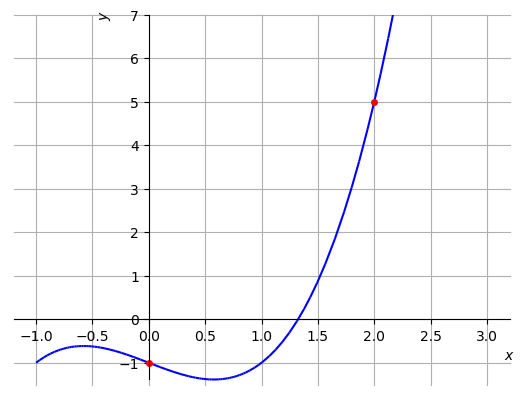
\includegraphics[width=0.7\textwidth]{./cap_lim/dados/fig_cap_lim_ex_teoint/fig_cap_lim_ex_teoint}
    \caption{Esboço do gráfico da função $f(x) = x^3-x-1$.}
    \label{fig:cap_lim_ex_teoint}
  \end{figure}
\end{ex}

\subsection*{Exercícios resolvidos}

\begin{exeresol}
  Encontre os pontos de continuidade da função
  \begin{equation}
    f(x) = \frac{|x|}{x}.
  \end{equation}
\end{exeresol}
\begin{resol}
  Observamos que a função é descontínua em $x=0$, pois não está definida neste ponto. Agora, para $x < 0$, temos
  \begin{equation}
    f(x) = \frac{|x|}{x} = \frac{-x}{x} = -1.
  \end{equation}
  Ou seja, para $x<0$ a função é constante igual a $-1$ e, portanto, contínua.

  Para $x > 0$, temos
  \begin{equation}
    f(x) = \frac{|x|}{x} = \frac{x}{x} = 1.
  \end{equation}
  I.e., para $x > 0$ a função é constante igual a $1$ e, portanto, contínua.

  Concluímos que $f(x)$ é contínua em $\mathbb{R}\setminus\{0\}$. Faça o esboço do gráfico desta função!
\end{resol}

\begin{exeresol}
  Encontre os pontos de continuidade da função
  \begin{equation}
    f(x) = \ln\left(\frac{x+1}{x-1}\right).
  \end{equation}
\end{exeresol}
\begin{resol}
  A função $f$ pode ser vista como a composição da função logaritmo natural $g(x) = \ln x$ com a função racional $\displaystyle h(x) = \frac{x+1}{x-1}$. Observamos que:
  \begin{enumerate}[a)]
  \item a função logaritmo natural é contínua em todo o seu domínio, i.e. $g$ é contínua para todo $x > 0$;
  \item a função racional $\displaystyle h(x) = \frac{x+1}{x-1}$ é contínua para todo $x\neq 1$.
  \end{enumerate}
  Lembrando que a composição de funções contínuas é contínua, temos que a função $f(x) = g(h(x))$ é contínua nos pontos de continuidade da função $h$ tais que $h(x) > 0$, i.e. para $x\neq 1$ e
  \begin{align}
    \frac{x+1}{x-1} > 0.
  \end{align}
  Fazendo o estudo de sinal
  \begin{center}
    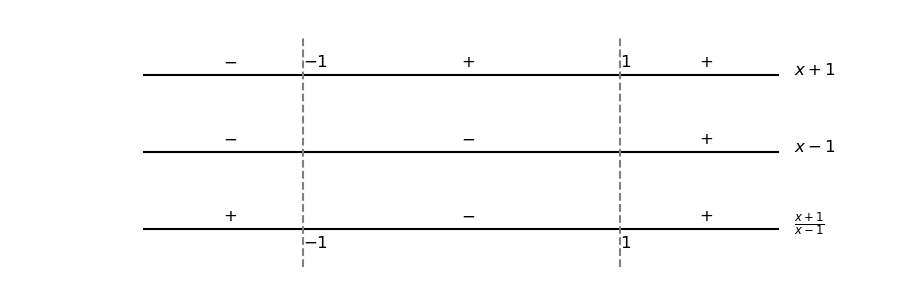
\includegraphics[width=0.8\textwidth]{./cap_lim/dados/fig_cap_lim_exeresol_estsinal/fig_cap_lim_exeresol_estsinal}
  \end{center}
  vemos que $h(x) > 0$ em $(-\infty, -1)\cup (1, \infty)$.

  Em resumo, $h$ é contínua em $(0, \infty)$ e $g$ é contínua e positiva em $(-\infty, -1)\cup (1, \infty)$. A função $f = (h\circ g)$ é contínua na interseção destes conjuntos, i.e. $f$ é contínua em $(1, \infty)$. 
\end{resol}

\subsection*{Exercícios}

\begin{exer}
  Encontre os pontos de continuidade da função
  \begin{equation}
    f(x) = \frac{x^3 - 27}{x^2 - 3x + 2}.
  \end{equation}
\end{exer}
\begin{resp}
  $\mathbb{R}\setminus\{1,2\}$.
\end{resp}

\begin{exer}
  Encontre os pontos de continuidade da função
  \begin{equation}
    f(x) = \sqrt{\frac{x^3 - 27}{x^2 - 3x + 2}}.
  \end{equation}
\end{exer}
\begin{resp}
  $(1, 2)\cup (3, \infty)$.
\end{resp}

\begin{exer}
  Calcule
  \begin{equation}
    \lim_{x\to \pi} \ln \left(\frac{\sen \frac{x}{2} - \cos x}{2}\right).
  \end{equation}
\end{exer}
\begin{resp}
  $0$
\end{resp}

\section{Limites e desigualdades}\label{cap_lim_sec_limdes}

Se $f$ e $g$ são funções tais que $f(x)<g(x)$ para todo $x$ em um certo intervalo aberto contendo $a$, exceto possivelmente em $x=a$, e existem os limites de $f$ e $g$ no ponto $x=a$, então
\begin{equation}
  \lim_{x\to a} f(x) \leq \lim_{x\to a} g(x).
\end{equation}
Observe que a tomada do limite não preserva a desigualdade estrita.

\begin{exer}
  As funções $f(x) = x^2/3$ e $g(x) = x^2/2$ são tais que $f(x) < g(x)$ para todo $x\neq 0$. Ainda, temos
  \begin{equation}
    \lim_{x\to 0} f(x) = 0\quad\text{e}\quad\lim_{x\to 0} g(x) = 0.
  \end{equation}
\end{exer}

\begin{obs}
  A preservação da desigualdade também ocorre para limites laterais. Mais precisamente, se $f$ e $g$ são funções tais que $f(x)<g(x)$ para todo $x < a$ e existem os limites lateral à esquerda de $f$ e $g$ no ponto $x=a$, então
  \begin{equation}
    \lim_{x\to a^-} f(x) \leq \lim_{x\to a^-} g(x).
  \end{equation}
  Vale o resultado análogo para limite lateral à direito. Escreva-o!
\end{obs}

\begin{ex}
  Vamos calcular o seguinte limite
  \begin{equation}
    \lim_{x\to \infty} e^x\sen x.
  \end{equation}

  \emconstrucao
\end{ex}


\subsection{Teorema do confronto}

\begin{teo}\normalfont{(Teorema do confronto)}\label{teo:confronto}
  Se $g(x) \leq f(x) \leq h(x)$ para todo $x$ em um intervalo aberto contendo $a$, exceto possivelmente em $x=a$, e
  \begin{equation}
    \lim_{x\to a} g(x) = \lim_{x\to a} h(x) = L,
  \end{equation}
  então
  \begin{equation}
    \lim_{x\to a} f(x) = L.
  \end{equation}
\end{teo}
\begin{dem}
  Da preservação da desigualdade, temos
  \begin{equation}
    \lim_{x\to a} g(x) \leq \lim_{x\to a} f(x) \leq \lim_{x\to a} h(x)
  \end{equation}
  donde
  \begin{equation}
    L \leq \lim_{x\to a} f(x) \leq L.
  \end{equation}
\end{dem}

\begin{exer}
  Toda função $f(x)$ tal que $-1+x^2/2 \leq f(x) \leq -1+x^2/3$, para todo $x\neq 0$, tem
  \begin{equation}
    \lim_{x\to 0} f(x) = -1.
  \end{equation}
\end{exer}

\begin{obs}
  O Teorema do confronto também se aplica a limites laterais.
\end{obs}

\begin{ex}\label{ex:senx}
  \begin{equation}
    \lim_{x\to 0} \sen x = 0.
  \end{equation}
  De fato, começamos assumindo $0<x<\pi/2$. Tomando $O = (0,0)$, $A=(1,0)$ e $P = (\cos x, \sen x)$, observamos que
  \begin{equation}
    \text{Área do triâng.} OAP < \text{Área do setor} OAP,
  \end{equation}
  i.e.
  \begin{equation}
    \frac{\sen x}{2} < \frac{x}{2} \Rightarrow \sen x < x,
  \end{equation}
  para todo $0< x < \pi/2$. 

  É certo que $\sen x < -x$ para $-\pi/2 < x < 0$. Com isso e o resultado acima, temos
  \begin{equation}\label{eq:senx0}
    \sen x \leq |x|,\quad -\pi/2 < x < \pi/2.
  \end{equation}

  Lembrando que $\sen x$ é uma função ímpar, temos
  \begin{equation}\label{eq:senx1}
    -|x| \leq -\sen x = \sen -x,\quad -\pi/2 < x < \pi/2.
  \end{equation}
  Logo, de \eqref{eq:senx0} e \eqref{eq:senx1}, temos
  \begin{equation}
    -|x| \leq \sen x \leq |x|.
  \end{equation}

  Por fim, como
  \begin{equation}
    \lim_{x\to 0} -|x| = \lim_{x\to 0} |x| = 0,
  \end{equation}
  do Teorema do confronto, concluímos
  \begin{equation}
    \lim_{x\to 0} \sen x = 0.
  \end{equation}
\end{ex}

\begin{obs}
  Do exemplo anterior (Exemplo \ref{ex:senx}), podemos mostrar que
\begin{equation}
  \lim_{x\to 0} \cos x = 1.
\end{equation}

De fato, da identidade trigonométrica de ângulo metade \eqref{eq:id_trig_cos_x2}
\begin{equation}
  \sen^2 \frac{x}{2} = \frac{1 - \cos x}{2}
\end{equation}
temos
\begin{equation}
  \cos x = 1 + 2\sen^2 \frac{x}{2}.
\end{equation}
Então, aplicando as regras de cálculo de limites, obtemos
\begin{align}
  \lim_{x\to 0} \cos x &= \lim_{x\to 0} \left[1 + 2\sen^2 \frac{x}{2}\right] \\
                       &= 1 + 2\left(\lim_{x\to 0} \sen \frac{x}{2}\right)^2.\label{eq:senx2}
\end{align}
Agora, fazemos a mudança de variável $y = x/2$. Neste caso, temos $y\to 0$ quando $x\to 0$ e, então
\begin{equation}
  \lim_{x\to 0} \sen \frac{x}{2} = \lim_{y\to 0} \sen y = 0.
\end{equation}
Então, retornando a equação \eqref{eq:senx2}, concluímos
\begin{equation}
  \lim_{x\to 0} \cos x = 1.
\end{equation}
\end{obs}

\subsection{Limites envolvendo $(\sen x)/x$}

Verificamos o seguinte resultado
\begin{equation}
  \lim_{x\to 0} \frac{\sen x}{x} = 1.
\end{equation}

Para verificarmos este resultado, calcularemos os limites laterais à esquerda e à direita. Começamos com o limite lateral a direita e assumimos $0<x<\pi/2$. Sendo os pontos $O=(0,0)$, $P=(\cos x,\sen x)$, $A = (1,0)$ e $T = (1, \tg x)$, observamos que
\begin{equation}
  \text{Área do triâng. } OAP < \text{Área do setor} OAP < \text{Área do triâng. } OAT.
\end{equation}
Ou seja, temos
\begin{equation}
  \frac{\sen x}{2} < \frac{x}{2} < \frac{\tg x}{2}.
\end{equation}
Multiplicando por $2$ e dividindo por $\sen x$\footnote{$\sen x > 0$ para todo $0< x < \pi/2$.}, obtemos
\begin{equation}
  1 < \frac{x}{\sen x} < \frac{1}{\cos x}.
\end{equation}
Tomando os recíprocos, temos
\begin{equation}
  1 > \frac{\sen x}{x} > \cos x.
\end{equation}
Agora, passando ao limite
\begin{equation}
  1 = \lim_{x\to 0^+} 1 \geq \lim_{x\to 0^+} \frac{\sen x}{x} \geq \lim_{x\to 0^+} \cos x = 1.
\end{equation}
Logo, concluímos que
\begin{equation}
  \lim_{x\to 0^+} \frac{\sen x}{x} = 1.
\end{equation}

Agora, usando o fato de que $\sen x/x$ é uma função par, temos
\begin{align}
  \lim_{x\to 0^-} \frac{\sen x}{x} &= \lim_{x\to 0^-} \frac{\sen(-x)}{-x} \\
  &= \lim_{x\to 0^+} \frac{\sen x}{x} = 1.
\end{align}

Calculados os limites laterais, concluímos o que queríamos.

\begin{ex}
  Com o resultado acima e as regras de cálculo de limites, temos
  \begin{equation}
    \lim_{x\to 0} \frac{\cos(x) - 1}{x} = 0.
  \end{equation}
  Veja o Exercício \ref{exer:lim_cosx_1}.
\end{ex}

% \begin{exer}
%   Pode-se mostrar que $|-x| \leq \sen x \leq |x|$ (veja a Figura \ref{fig:}). Ainda, como
%   \begin{equation}
%     \lim_{x\to 0} -|x| = \lim_{x\to 0} |x| = 0,
%   \end{equation}
%   temos, pelo Teorema do confronto (Teorema \ref{teo:confronto}),
%   \begin{equation}
%     \lim_{x\to 0} \sen x = 0.
%   \end{equation}
% \end{exer}

\subsection*{Exercícios}

\begin{exer}
  Supondo que $1-x^2/3 \leq u(x) \leq 1-x^2/2$ para todo $x\neq 0$, determine o $\lim_{x\to 0} u(x)$.
\end{exer}
\begin{resp}
  $1$
\end{resp}

\begin{exer}
  Calcule
  \begin{equation}
    \lim_{x\to 0} \frac{\sen 3x}{6x}.
  \end{equation}
\end{exer}
\begin{resp}
  $0$
\end{resp}

\begin{exer}\label{exer:lim_cosx_1}
  Calcule
  \begin{equation}
    \lim_{x\to 0} \frac{\cos(x)-1}{x}.
  \end{equation}
\end{exer}
\begin{resp}
  $0$
\end{resp}

\begin{exer}
  Calcule
  \begin{equation}
    \lim_{x\to 0} \frac{\cos(3x)-1}{6x}.
  \end{equation}
\end{exer}
\begin{resp}
  $\frac{1}{2}$
\end{resp}

\emconstrucao

\section{Exercícios finais}\label{cap_lim_sec_exfinal}

\begin{exer}
  Calcule
  \begin{equation}
    \lim_{x\to 1^+} \ln\left(\frac{x+1}{x-1}\right).
  \end{equation}
\end{exer}
\begin{resp}
  $\infty$
\end{resp}

